\documentclass[a4paper,12pt]{article}

% При наличии T2A файл можно собирать pdfLaTeX; для рабочей среды подходит XeLaTeX.
\usepackage{iftex}
\ifPDFTeX
    \usepackage[T2A]{fontenc}
    \usepackage[utf8]{inputenc}
    \usepackage[russian]{babel}
\else
    \usepackage{fontspec}
    \usepackage{polyglossia}
    \setmainlanguage{russian}
    \setmainfont{DejaVu Serif}
    \newfontfamily\cyrillicfonttt{DejaVu Sans Mono}
\fi
\usepackage{amsmath,amssymb,mathtools}
\usepackage{graphicx,booktabs}
\usepackage{geometry}
\usepackage{indentfirst}
\usepackage{microtype}
\usepackage{ragged2e}
\geometry{left=2.5cm,right=2.5cm,top=2.1cm,bottom=2.1cm}
\setlength{\parindent}{0.7cm}
\setlength{\parskip}{0pt}
\setlength{\abovedisplayskip}{9pt plus 2pt minus 3pt}
\setlength{\belowdisplayskip}{9pt plus 2pt minus 3pt}
\setlength{\abovedisplayshortskip}{4pt plus 2pt minus 2pt}
\setlength{\belowdisplayshortskip}{6pt plus 2pt minus 2pt}
\linespread{0.97}
\emergencystretch=4em
\tolerance=3000

\title{Восстановление относительных траекторий группы из четырёх космических аппаратов по геометрии наблюдаемой проекции}
\author{И.~В.~Шимановская}
\date{Рабочий черновик для обсуждения}

\begin{document}
\justifying
\setlength{\parindent}{0.7cm}
\maketitle

\section{Постановка задачи}

В выполненной работе исходной являлась пространственная конфигурация четырёх космических аппаратов (КА): опорный аппарат и три ведомых образуют квадрат в орбитальной системе отсчёта (ОСО). Для удержания этого квадрата строилось управление, после чего вычислялась его проекция для наземного наблюдателя. Полученный интервал, на котором проекция удовлетворяет критериям квадрата, существенно короче интервала удержания пространственной конфигурации. Поэтому далее целесообразно изменить порядок построения: сначала задать необходимую наблюдаемую геометрию, а затем найти соответствующие ей относительные траектории.

На первом этапе рассмотрим те же четыре КА. Опорный аппарат считается одной из вершин видимого квадрата, а его орбита и положение наземного наблюдателя заданы. В расчётный момент требуется восстановить относительные положения трёх ведомых аппаратов по точкам их изображения. Затем нужно определить начальные относительные скорости, при которых проекция остаётся близкой к квадрату на заданном интервале $I=[t_-,t_+]$. Предпочтительным является движение без тяги на этом интервале; если для формирования или поддержания конфигурации необходимы манёвры, их величину следует оценивать отдельно.

Здесь важно различать две постановки. Заданный квадрат означает, что координаты всех трёх ведомых точек в картинной плоскости фиксированы, включая масштаб и ориентацию изображения. Критерий близости к квадрату ограничивает длины сторон, диагонали и углы, но сам по себе не фиксирует ни угловой размер, ни поворот фигуры. Ниже сначала решается задача с заданными точками, затем записываются критерии формы и условие минимального расхода управления.

\section{Наблюдаемая проекция и относительное положение}

\subsection{Геометрия наблюдения}

Введём геоцентрическую инерциальную систему с осью $E_Z$, направленной вдоль оси вращения Земли. Землю при построении видимости считаем сферой радиуса $R_E$. В расчётном примере принимаем
\begin{equation}
\begin{gathered}
 R_E=6371\ {\rm км},\quad \mu=3{,}986004\cdot10^5\ {\rm км^3/с^2},
 \quad J_2=1{,}08263\cdot10^{-3},\\
 \Omega_E=7{,}2921150\cdot10^{-5}\ {\rm рад/с},\quad
 h_0=630\ {\rm км},\quad i_0=97{,}8^\circ,\\
 \varphi_{\rm obs}=25{,}3026^\circ,\qquad
 \ell_{\rm obs}=51{,}5132^\circ.
\end{gathered}
\label{eq:parameters}
\end{equation}
Здесь $\mu$ --- гравитационный параметр Земли, $J_2$ --- коэффициент второй зональной гармоники, $\Omega_E$ --- угловая скорость вращения Земли, $\varphi_{\rm obs}$ и $\ell_{\rm obs}$ --- широта и долгота наблюдателя. В формулах ниже длины и ускорения следует вычислять в согласованных единицах; значения параметров не являются ограничением предлагаемого метода.

Пусть в момент $t_0$ угол поворота нулевого меридиана относительно инерциальной оси $E_X$ равен $\Theta_0$. Обозначим $\Lambda(t)=\ell_{\rm obs}+\Theta_0+\Omega_E(t-t_0)$. Для неподвижного на поверхности наблюдателя его радиус-вектор, скорость и ускорение в инерциальной системе находятся без обращения к эфемеридам:
\begin{equation}
 \mathbf R(t)=R_E
 \begin{pmatrix}
  \cos\varphi_{\rm obs}\cos\Lambda(t)\\
  \cos\varphi_{\rm obs}\sin\Lambda(t)\\
  \sin\varphi_{\rm obs}
 \end{pmatrix},\qquad
 \dot{\mathbf R}=\Omega_E\mathbf E_Z\times\mathbf R,\quad
 \ddot{\mathbf R}=\Omega_E\mathbf E_Z\times\dot{\mathbf R}.
 \label{eq:observer_state}
\end{equation}
Выбор $\Theta_0=0$ лишь задаёт ориентацию инерциальной оси $E_X$ в момент $t_0$.

Для явного расчёта номинальной орбиты пока примем круговое двухтельное движение. Положим $a_0=R_E+h_0$, $n=\sqrt{\mu/a_0^3}$ и $u(t)=u_0+n(t-t_0)$. Введём матрицы поворота
\begin{equation}
 R_z(\Omega)=
 \begin{pmatrix}\cos\Omega&-\sin\Omega&0\\
                 \sin\Omega& \cos\Omega&0\\0&0&1\end{pmatrix},
 \qquad
 R_x(i)=
 \begin{pmatrix}1&0&0\\0&\cos i&-\sin i\\0&\sin i&\cos i\end{pmatrix}.
 \label{eq:rotation_matrices}
\end{equation}
Здесь $\Omega_0$ --- долгота восходящего узла, $u_0$ --- аргумент широты опорного КА в момент $t_0$. Его положение и скорость равны
\begin{equation}
\begin{aligned}
 \mathbf r_0(t)&=a_0R_z(\Omega_0)R_x(i_0)
       (\cos u(t),\,\sin u(t),\,0)^T,\\
 \dot{\mathbf r}_0(t)&=a_0nR_z(\Omega_0)R_x(i_0)
       (-\sin u(t),\,\cos u(t),\,0)^T.
\end{aligned}
\label{eq:reference_orbit}
\end{equation}
Если $t_0$ назначен моментом зенитного пролёта, то
$\mathbf r_0(t_0)=a_0\mathbf R(t_0)/R_E$. Сравнение третьих компонент
\eqref{eq:observer_state} и \eqref{eq:reference_orbit}, а затем их долгот
даёт конструктивный выбор орбиты:
\begin{equation}
 \sin u_0=\frac{\sin\varphi_{\rm obs}}{\sin i_0},\qquad
 \Omega_0=\Lambda(t_0)-
   \operatorname{atan2}(\cos i_0\sin u_0,\,\cos u_0).
 \label{eq:zenith_orbit}
\end{equation}
Для восходящего пересечения широты берётся ветвь с $\cos u_0>0$;
существует и нисходящая ветвь. Равенство возможно лишь при
$|\sin\varphi_{\rm obs}|\leq|\sin i_0|$. Формулы
\eqref{eq:observer_state}--\eqref{eq:zenith_orbit} полностью задают
геометрию одного номинального пролёта; при ином времени $t_0$ меняется
лишь общая ориентация относительно инерциальной системы.

Построим орбитальную систему отсчёта (ОСО) с началом в опорном КА:
\begin{equation}
 \mathbf e_x=\frac{\mathbf r_0}{\|\mathbf r_0\|},\qquad
 \mathbf e_z=\frac{\mathbf r_0\times\dot{\mathbf r}_0}
                   {\|\mathbf r_0\times\dot{\mathbf r}_0\|},\qquad
 \mathbf e_y=\mathbf e_z\times\mathbf e_x,\qquad
 B=[\mathbf e_x\ \mathbf e_y\ \mathbf e_z].
 \label{eq:orbital_basis}
\end{equation}
Следовательно, $B^TB=I_3$, а $B^T$ переводит инерциальный вектор в ОСО.
Для круговой орбиты \eqref{eq:reference_orbit}
$\dot{\mathbf e}_x=n\mathbf e_y$,
$\dot{\mathbf e}_y=-n\mathbf e_x$ и $\dot{\mathbf e}_z=0$; поэтому
\begin{equation}
 \dot B=B
 \begin{pmatrix}0&-n&0\\n&0&0\\0&0&0\end{pmatrix}.
 \label{eq:basis_derivative}
\end{equation}
Для ведомого КА с индексом $i=1,2,3$ введём его относительное
положение $\boldsymbol\rho_i=(x_i,y_i,z_i)^T$:
\begin{equation}
    \mathbf r_i(t)=\mathbf r_0(t)+B(t)\boldsymbol\rho_i(t),
    \qquad
    \boldsymbol\rho_i(t)=
    \begin{pmatrix}x_i(t)\\y_i(t)\\z_i(t)\end{pmatrix}.
    \label{eq:relative_position}
\end{equation}

Введём направление на опорный аппарат и расстояние до него:
\begin{equation}
    D_0(t)=\|\mathbf r_0(t)-\mathbf R(t)\|,
    \qquad
    \mathbf s_0(t)=\frac{\mathbf r_0(t)-\mathbf R(t)}{D_0(t)}.
    \label{eq:chief_sight}
\end{equation}
Для однозначной ориентации картинной плоскости сначала спроецируем
трансверсальную ось ОСО на плоскость, перпендикулярную $\mathbf s_0$:
\begin{equation}
 \mathbf w=\mathbf e_y-(\mathbf e_y\cdot\mathbf s_0)\mathbf s_0,\qquad
 \mathbf e_\xi=\frac{\mathbf w}{\|\mathbf w\|},\qquad
 \mathbf e_\eta=\mathbf s_0\times\mathbf e_\xi.
 \label{eq:image_basis}
\end{equation}
Векторы $(\mathbf e_\xi,\mathbf e_\eta,\mathbf s_0)$ ортонормированы и
образуют правую тройку. Если $\|\mathbf w\|=0$, вместо $\mathbf e_y$
надо выбрать другую ось, не параллельную $\mathbf s_0$; в окрестности
зенитного пролёта этой особенности нет. Вектор от наблюдателя к $i$-му
аппарату равен
\begin{equation}
    \boldsymbol\ell_i(t)=\mathbf r_i(t)-\mathbf R(t)
    =D_0(t)\mathbf s_0(t)+B(t)\boldsymbol\rho_i(t).
    \label{eq:line_of_sight}
\end{equation}
Выведем правило проекции. Единичное направление на аппарат есть
$\mathbf s_i=\boldsymbol\ell_i/\|\boldsymbol\ell_i\|$.
Касательная к единичной сфере плоскость в точке $\mathbf s_0$
описывается равенством $\mathbf q\cdot\mathbf s_0=1$. Луч от начала
небесной сферы имеет вид $\mathbf q=\beta\mathbf s_i$; подстановка в
уравнение плоскости даёт
$\beta=1/(\mathbf s_i\cdot\mathbf s_0)$. Координаты точки пересечения
в базисе \eqref{eq:image_basis} поэтому равны
\begin{equation}
 \xi_i=\frac{\mathbf s_i\cdot\mathbf e_\xi}
              {\mathbf s_i\cdot\mathbf s_0}
      =\frac{\boldsymbol\ell_i\cdot\mathbf e_\xi}
              {\boldsymbol\ell_i\cdot\mathbf s_0},
 \qquad
 \eta_i=\frac{\mathbf s_i\cdot\mathbf e_\eta}
              {\mathbf s_i\cdot\mathbf s_0}
      =\frac{\boldsymbol\ell_i\cdot\mathbf e_\eta}
              {\boldsymbol\ell_i\cdot\mathbf s_0}.
    \label{eq:gnomonic}
\end{equation}
Для опорного КА $\xi_0=\eta_0=0$. Формулы применяются, если знаменатель положителен, то есть направление на ведомый аппарат попадает в используемую полусферу проекции.

\subsection{Обратное построение точки изображения}

Предположим, что в момент $t$ требуются координаты изображения $(\xi_i^*,\eta_i^*)$. Сначала распишем числители и знаменатель проекции через компоненты относительного положения. Для каждой оси $k\in\{x,y,z\}$ обозначим
\begin{equation}
    a_k=\mathbf e_\xi\cdot\mathbf e_k,\qquad
    b_k=\mathbf e_\eta\cdot\mathbf e_k,\qquad
    c_k=\mathbf s_0\cdot\mathbf e_k.
    \label{eq:frame_coefficients}
\end{equation}
Вектор $D_0\mathbf s_0$ ортогонален обеим осям картинной плоскости. Поэтому для $\boldsymbol\rho_i=(x_i,y_i,z_i)^T$ из \eqref{eq:line_of_sight} имеем
\begin{equation}
\begin{aligned}
    \boldsymbol\ell_i\cdot\mathbf e_\xi
        &=a_xx_i+a_yy_i+a_zz_i,\\
    \boldsymbol\ell_i\cdot\mathbf e_\eta
        &=b_xx_i+b_yy_i+b_zz_i,\\
    \boldsymbol\ell_i\cdot\mathbf s_0
        &=D_0+c_xx_i+c_yy_i+c_zz_i.
\end{aligned}
    \label{eq:projection_components}
\end{equation}
В частности, требование $\xi_i=\xi_i^*$ означает равенство $a_xx_i+a_yy_i+a_zz_i=\xi_i^*(D_0+c_xx_i+c_yy_i+c_zz_i)$. Перенося слагаемые с координатами в левую часть и повторяя ту же операцию для $\eta_i$, получаем два линейных уравнения:
\begin{equation}
    \begin{cases}
    (a_x-\xi_i^*c_x)x_i+(a_y-\xi_i^*c_y)y_i
                           +(a_z-\xi_i^*c_z)z_i=D_0\xi_i^*,\\
    (b_x-\eta_i^*c_x)x_i+(b_y-\eta_i^*c_y)y_i
                           +(b_z-\eta_i^*c_z)z_i=D_0\eta_i^*.
    \end{cases}
    \label{eq:two_constraints}
\end{equation}
В компактном виде левая часть первого уравнения равна $(\mathbf e_\xi-\xi_i^*\mathbf s_0)^TB\boldsymbol\rho_i$; второе устроено аналогично. Все векторы базиса и $D_0$ берутся в один момент времени. Система \eqref{eq:two_constraints} даёт два скалярных условия на три координаты. Пока одна координата не выбрана дополнительно, единственного положения нет.

Покажем решение обычной линейной системы. Для краткости введём $A_{\xi k}=a_k-\xi_i^*c_k$ и $A_{\eta k}=b_k-\eta_i^*c_k$. Выберем $x_i$ свободным и перенесём содержащие его слагаемые вправо:
\begin{equation}
    \begin{pmatrix}A_{\xi y}&A_{\xi z}\\
                    A_{\eta y}&A_{\eta z}\end{pmatrix}
    \begin{pmatrix}y_i\\z_i\end{pmatrix}
    =\begin{pmatrix}R_{\xi i}\\R_{\eta i}\end{pmatrix},
    \quad
    \begin{cases}
    R_{\xi i}=D_0\xi_i^*-A_{\xi x}x_i,\\
    R_{\eta i}=D_0\eta_i^*-A_{\eta x}x_i.
    \end{cases}
    \label{eq:two_by_two}
\end{equation}
Если $\Delta_i=A_{\xi y}A_{\eta z}-A_{\xi z}A_{\eta y}\ne0$, получаем
\begin{equation}
    y_i=\frac{A_{\eta z}R_{\xi i}-A_{\xi z}R_{\eta i}}{\Delta_i},
    \qquad
    z_i=\frac{A_{\xi y}R_{\eta i}-A_{\eta y}R_{\xi i}}{\Delta_i}.
    \label{eq:explicit_yz}
\end{equation}
Таким образом, выбор $x_i$ задаёт $y_i$ и $z_i$ по формулам \eqref{eq:explicit_yz}. При $\Delta_i=0$ именно такой выбор свободной координаты неудобен: следует решить два уравнения относительно другой пары координат. Геометрическое решение через луч, приведённое ниже, не требует выбирать заранее, какая из трёх координат будет свободной.

Действительно, равенства для $\xi_i^*$ и $\eta_i^*$ означают, что поперечные компоненты $\boldsymbol\ell_i$ равны соответственно $\xi_i^*$ и $\eta_i^*$ от его компоненты вдоль $\mathbf s_0$. Обозначим эту последнюю через $\lambda_i$:
\begin{equation}
    \lambda_i=\boldsymbol\ell_i\cdot\mathbf s_0>0,
    \qquad
    \mathbf u_i=\mathbf s_0+\xi_i^*\mathbf e_\xi+\eta_i^*\mathbf e_\eta.
\end{equation}
Разложение $\boldsymbol\ell_i$ по ортонормированному базису $(\mathbf s_0,\mathbf e_\xi,\mathbf e_\eta)$ даёт $\boldsymbol\ell_i=\lambda_i\mathbf u_i$. С учётом $\mathbf r_0-\mathbf R=D_0\mathbf s_0$ отсюда последовательно получаются все положения с заданной проекцией:
\begin{equation}
    \mathbf r_i=\mathbf R+\lambda_i\mathbf u_i,
    \qquad
    \boldsymbol\rho_i
    =B^T\left[(\lambda_i-D_0)\mathbf s_0
       +\lambda_i\xi_i^*\mathbf e_\xi
       +\lambda_i\eta_i^*\mathbf e_\eta\right].
    \label{eq:inverse_ray}
\end{equation}
Параметр $\lambda_i$ представляет собой составляющую дальности по направлению $\mathbf s_0$; физическое расстояние от наблюдателя равно $\lambda_i\sqrt{1+(\xi_i^*)^2+(\eta_i^*)^2}$. Поэтому без дополнительных условий нельзя восстановить единственную пространственную конфигурацию даже в один момент времени.

Один из способов дополнить эти два уравнения --- назначить каждому КА радиус начальной орбиты $r_i^*=R_E+h_i$. Тогда третьим условием становится $\|\mathbf r_i\|^2=(r_i^*)^2$. Подставляя $\mathbf r_i=\mathbf R+\lambda_i\mathbf u_i$, получаем квадратное уравнение именно для оставшейся дальности:
\begin{equation}
    \|\mathbf u_i\|^2\lambda_i^2
       +2(\mathbf R\cdot\mathbf u_i)\lambda_i
       +\|\mathbf R\|^2-(r_i^*)^2=0.
    \label{eq:altitude_quadratic}
\end{equation}
Если луч пересекает требуемую сферу впереди наблюдателя, нужный положительный корень равен
\begin{equation}
    \lambda_i=
    \frac{-\mathbf R\cdot\mathbf u_i+
      \sqrt{(\mathbf R\cdot\mathbf u_i)^2+
       \|\mathbf u_i\|^2\bigl((r_i^*)^2-\|\mathbf R\|^2\bigr)}}
       {\|\mathbf u_i\|^2}.
    \label{eq:altitude_range}
\end{equation}
Это определяет начальное положение, но не начальную скорость. Одинаковая высота всех аппаратов является удобным пробным условием, а не следствием критерия проекции. Её выбор необходимо проверять по дальнейшему движению и сближениям; можно также назначить разные $h_i$ и тем самым исследовать другие начальные конфигурации.

Для проверки результата рассмотрим расчётный момент $t_0$, когда опорный КА находится в зените наблюдателя и выбранный базис проекции совпадает с осями ОСО: $\mathbf s_0=\mathbf e_x$, $\mathbf e_\xi=\mathbf e_y$, $\mathbf e_\eta=\mathbf e_z$. Тогда $\boldsymbol\ell_i=(D_0+x_i)\mathbf e_x+y_i\mathbf e_y+z_i\mathbf e_z$, а исходные дроби \eqref{eq:gnomonic} становятся
\begin{equation}
    \xi_i=\frac{y_i}{D_0+x_i},
    \qquad
    \eta_i=\frac{z_i}{D_0+x_i}.
    \label{eq:zenith_projection}
\end{equation}
Приравнивая их заданным $\xi_i^*,\eta_i^*$, сразу находим
\begin{equation}
    y_i=(D_0+x_i)\xi_i^*,
    \qquad
    z_i=(D_0+x_i)\eta_i^*,
    \qquad D_0+x_i>0.
    \label{eq:zenith_inverse}
\end{equation}
Можно выбрать $x_i$, после чего две другие координаты находятся однозначно. Условие $x_i=0$ восстанавливает квадрат в плоскости $Oyz$, использованный ранее, но из геометрии изображения это условие не следует.

\subsection{Четыре вершины квадрата}

Положим $\mathbf p_0^*=(0,0)^T$ и для определённости зададим в картинной плоскости квадрат со стороной $\alpha>0$:
\begin{equation}
    \mathbf p_1^*=(\alpha,0)^T,
    \qquad
    \mathbf p_2^*=(\alpha,\alpha)^T,
    \qquad
    \mathbf p_3^*=(0,\alpha)^T.
    \label{eq:target_square}
\end{equation}
Параметр $\alpha$ здесь является длиной стороны в гномонических координатах, а не углом в радианах; соответствующий угловой размер около центра равен $\arctan\alpha$. Если при зенитном пролёте и $x_i=0$ нужно получить пространственную сторону $L$, следует принять $\alpha=L/D_0$. В частности, при $D_0=630$~км и $L=20$~км получаем $\alpha\simeq0{,}03175$ и $\arctan\alpha\simeq1{,}82^\circ$.

В момент $t_0$ из \eqref{eq:zenith_inverse} следует семейство пространственных конфигураций
\begin{equation}
    \boldsymbol\rho_{10}=\begin{pmatrix}x_1\\\alpha(D_0+x_1)\\0\end{pmatrix},
    \quad
    \boldsymbol\rho_{20}=\begin{pmatrix}x_2\\\alpha(D_0+x_2)\\\alpha(D_0+x_2)\end{pmatrix},
    \quad
    \boldsymbol\rho_{30}=\begin{pmatrix}x_3\\0\\\alpha(D_0+x_3)\end{pmatrix}.
    \label{eq:four_spacecraft_initial_positions}
\end{equation}
При любом допустимом наборе $x_1,x_2,x_3$ проекция в этот момент будет одним и тем же квадратом. Поэтому для трёх ведомых КА имеются три свободные радиальные координаты, а не одна общая для всей группы.

Если требовать лишь форму квадрата, не назначая его масштаб и поворот, можно положить
\begin{equation}
    \mathbf p_1=(a,b)^T,\qquad
    \mathbf p_3=(-b,a)^T,\qquad
    \mathbf p_2=(a-b,a+b)^T.
    \label{eq:free_square}
\end{equation}
Параметры $a,b$ отвечают за масштаб и ориентацию, а $\lambda_1,\lambda_2,\lambda_3$ --- за положение КА вдоль трёх лучей. Если требования к сторонам, диагоналям и углам заданы с допусками, множество допустимых изображений ещё шире, чем семейство точных квадратов \eqref{eq:free_square}. Утверждение «два уравнения на три координаты» относится именно к заданной точке изображения каждого КА, а не ко всей системе критериев близости к квадрату.

\subsection{Проверяемые показатели формы и видимости}
\label{sec:shape_criteria}

В каждый момент вычислим фактические точки изображения
$\mathbf p_j(t)=(\xi_j(t),\eta_j(t))^T$, $j=0,1,2,3$, по
\eqref{eq:relative_position}--\eqref{eq:gnomonic}. Для опорной вершины
$\mathbf p_0=(0,0)^T$. Индексы вершин далее считаются по модулю $4$,
в порядке обхода границы четырёхугольника. Длины четырёх сторон,
их среднее и длины двух диагоналей задаются без выбора масштаба:
\begin{equation}
\begin{gathered}
 b_j=\|\mathbf p_{j+1}-\mathbf p_j\|,\qquad
 \bar b=\frac14\sum_{j=0}^{3}b_j,\\
 d_1=\|\mathbf p_2-\mathbf p_0\|,\qquad
 d_2=\|\mathbf p_3-\mathbf p_1\|.
\end{gathered}
\label{eq:side_diagonal_definitions}
\end{equation}
При ненулевых сторонах внутренний угол у вершины $j$ равен
\begin{equation}
 \gamma_j=\arccos\!\left(
 \frac{(\mathbf p_{j-1}-\mathbf p_j)^T
       (\mathbf p_{j+1}-\mathbf p_j)}
      {b_{j-1}b_j}\right).
 \label{eq:interior_angles}
\end{equation}
В численном вычислении аргумент $\arccos$ следует ограничивать
отрезком $[-1,1]$, чтобы округление не породило ошибку вычисления.
По этим величинам получаем три безразмерных или угловых показателя:
\begin{equation}
 \varepsilon_b=\frac{\max_j|b_j-\bar b|}{\bar b},\qquad
 \varepsilon_d=\frac{2|d_1-d_2|}{d_1+d_2},\qquad
 \varepsilon_\gamma=\max_j\left|\gamma_j-\frac{\pi}{2}\right|.
 \label{eq:shape_errors}
\end{equation}
Для квадрата все три равны нулю. Показатель
$\varepsilon_\gamma$ измеряется в радианах, если углы подставлены
в радианах; допуск $10^\circ$ при вычислении означает $\pi/18$.
Деление в \eqref{eq:shape_errors} предполагает $\bar b>0$ и
$d_1+d_2>0$. Дополнительно проверяем, что четыре вершины
образуют простой выпуклый контур с назначенным порядком обхода,
например, определители
$\det[\mathbf p_{j+1}-\mathbf p_j,\,
       \mathbf p_{j+2}-\mathbf p_{j+1}]$
все строго положительны для ориентации
\eqref{eq:target_square}. Эта проверка исключает самопересечение
или перестановку номеров вершин.

Для доступности наземному наблюдателю введём единичные направления
$\mathbf s_j=(\mathbf r_j-\mathbf R)/\|\mathbf r_j-\mathbf R\|$
и местную вертикаль $\mathbf R/R_E$. Угол места есть угол направления
на КА над плоскостью горизонта:
\begin{equation}
 h_j=\arcsin\!\left(\mathbf s_j\cdot\frac{\mathbf R}{R_E}\right),
 \qquad j=0,1,2,3.
 \label{eq:elevation}
\end{equation}
Например, для рассматриваемого сценария можно принять
$h_{\min}=15^\circ$,
$\varepsilon_{b,\max}=\varepsilon_{d,\max}=0{,}10$,
$\varepsilon_{\gamma,\max}=10^\circ$. Тогда в пределах
проверяемого промежутка $I_{\rm check}$ множество допустимых
моментов определяется непосредственно формулами
\begin{equation}
\begin{split}
 \mathcal T_{\rm obs}=\{t\in I_{\rm check}:\ &
 \min_{0\leq j\leq3} h_j(t)\geq h_{\min},\\
 &\varepsilon_b(t)\leq\varepsilon_{b,\max},\
 \varepsilon_d(t)\leq\varepsilon_{d,\max},\
 \varepsilon_\gamma(t)\leq\varepsilon_{\gamma,\max}\}.
\end{split}
\label{eq:observable_set}
\end{equation}
При поиске рабочего интервала $I$ следует выбирать связную
компоненту $\mathcal T_{\rm obs}$, а не предполагать заранее,
что допустимые моменты всегда образуют один интервал.
Если размер изображения также предписан, к
\eqref{eq:observable_set} добавляется ограничение на $\bar b$
или на расстояние от фактических $\mathbf p_i$ до
$\mathbf p_i^*$ из \eqref{eq:target_square}.

\section{Траектории при заданной проекции}

\subsection{Кинематическое семейство траекторий}

Пусть теперь требуемые координаты $\xi_i^*(t),\eta_i^*(t)$ заданы как функции времени. Тогда формула \eqref{eq:inverse_ray} остаётся справедливой в каждый момент при некоторой функции $\lambda_i(t)>0$:
\begin{equation}
    \mathbf r_i(t)=\mathbf R(t)+\lambda_i(t)\mathbf u_i(t),
    \qquad
    \mathbf u_i(t)=\mathbf s_0(t)+\xi_i^*(t)\mathbf e_\xi(t)
                             +\eta_i^*(t)\mathbf e_\eta(t).
    \label{eq:kinematic_trajectory}
\end{equation}
При дифференцировании $\mathbf u_i$ надо учитывать движение наблюдателя и поворот базиса изображения. Например,
\begin{equation}
    \dot{\mathbf u}_i=\dot{\mathbf s}_0
        +\dot\xi_i^*\mathbf e_\xi+\xi_i^*\dot{\mathbf e}_\xi
        +\dot\eta_i^*\mathbf e_\eta+\eta_i^*\dot{\mathbf e}_\eta.
    \label{eq:direction_derivative}
\end{equation}
Здесь все производные базисных векторов определяются заданной
геометрией, а не являются новыми управляющими переменными.
Например, положив
$\mathbf d_0=\mathbf r_0-\mathbf R$ и
$\mathbf v_0^{\rm los}=\dot{\mathbf r}_0-\dot{\mathbf R}$,
из $D_0=\|\mathbf d_0\|$, $\mathbf s_0=\mathbf d_0/D_0$
получаем
\begin{equation}
 \dot D_0=\mathbf s_0\cdot\mathbf v_0^{\rm los},\qquad
 \dot{\mathbf s}_0=
 \frac{\bigl(I_3-\mathbf s_0\mathbf s_0^T\bigr)
                  \mathbf v_0^{\rm los}}{D_0}.
 \label{eq:sight_derivative}
\end{equation}
Далее для $\mathbf w$ из \eqref{eq:image_basis} обозначим
$g=\mathbf e_y\cdot\mathbf s_0$. По правилу произведения
\begin{equation}
\begin{aligned}
 \dot g&=\dot{\mathbf e}_y\cdot\mathbf s_0+
                  \mathbf e_y\cdot\dot{\mathbf s}_0,\\
 \dot{\mathbf w}&=\dot{\mathbf e}_y-\dot g\,\mathbf s_0
                                -g\,\dot{\mathbf s}_0,\\
 \dot{\mathbf e}_\xi
   &=\frac{(I_3-\mathbf e_\xi\mathbf e_\xi^T)
                   \dot{\mathbf w}}{\|\mathbf w\|},\qquad
 \dot{\mathbf e}_\eta
   =\dot{\mathbf s}_0\times\mathbf e_\xi
                   +\mathbf s_0\times\dot{\mathbf e}_\xi .
\end{aligned}
\label{eq:image_basis_derivative}
\end{equation}
Для ускорения в \eqref{eq:required_acceleration} нужна также
\begin{equation}
\begin{aligned}
 \ddot{\mathbf u}_i={}&\ddot{\mathbf s}_0
   +\ddot\xi_i^*\mathbf e_\xi
   +2\dot\xi_i^*\dot{\mathbf e}_\xi
   +\xi_i^*\ddot{\mathbf e}_\xi\\
   &+\ddot\eta_i^*\mathbf e_\eta
   +2\dot\eta_i^*\dot{\mathbf e}_\eta
   +\eta_i^*\ddot{\mathbf e}_\eta.
\end{aligned}
\label{eq:direction_second_derivative}
\end{equation}
Её геометрические слагаемые можно вычислить
дифференцированием \eqref{eq:sight_derivative} и
\eqref{eq:image_basis_derivative}. В частности, если
$\mathbf a_0^{\rm los}=\ddot{\mathbf r}_0-\ddot{\mathbf R}$,
то
\begin{equation}
\begin{aligned}
 \ddot D_0&=\mathbf s_0\cdot\mathbf a_0^{\rm los}
       +\frac{\|\mathbf v_0^{\rm los}\|^2-\dot D_0^2}{D_0},\\
 \ddot{\mathbf s}_0
   &=\frac{\mathbf a_0^{\rm los}
           -\ddot D_0\mathbf s_0
           -2\dot D_0\dot{\mathbf s}_0}{D_0}.
\end{aligned}
\label{eq:sight_second_derivative}
\end{equation}
Для воспроизведения оставшихся производных удобно использовать
$N=\|\mathbf w\|$ и уже известное $g$:
\begin{equation}
\begin{aligned}
 \ddot g&=\ddot{\mathbf e}_y\cdot\mathbf s_0
   +2\dot{\mathbf e}_y\cdot\dot{\mathbf s}_0
   +\mathbf e_y\cdot\ddot{\mathbf s}_0,\\
 \ddot{\mathbf w}&=\ddot{\mathbf e}_y-\ddot g\,\mathbf s_0
   -2\dot g\,\dot{\mathbf s}_0-g\,\ddot{\mathbf s}_0,\\
 \dot N&=\mathbf e_\xi\cdot\dot{\mathbf w},\\
 \ddot{\mathbf e}_\xi
   &=\frac{(I_3-\mathbf e_\xi\mathbf e_\xi^T)
                    \ddot{\mathbf w}}{N}
     -\frac{2\dot N}{N}\dot{\mathbf e}_\xi
     -\|\dot{\mathbf e}_\xi\|^2\mathbf e_\xi,\\
 \ddot{\mathbf e}_\eta
   &=\ddot{\mathbf s}_0\times\mathbf e_\xi
     +2\dot{\mathbf s}_0\times\dot{\mathbf e}_\xi
     +\mathbf s_0\times\ddot{\mathbf e}_\xi.
\end{aligned}
\label{eq:image_basis_second_derivative}
\end{equation}
На круговой орбите $\ddot{\mathbf e}_y=-n^2\mathbf e_y$
из \eqref{eq:basis_derivative}, так что в формулах
\eqref{eq:sight_derivative}--\eqref{eq:image_basis_second_derivative}
не остаётся неопределённых величин.
После дифференцирования получаем необходимые скорость и ускорение:
\begin{align}
    \dot{\mathbf r}_i&=\dot{\mathbf R}+\dot\lambda_i\mathbf u_i
                                    +\lambda_i\dot{\mathbf u}_i,\label{eq:required_velocity}\\
    \ddot{\mathbf r}_i&=\ddot{\mathbf R}+\ddot\lambda_i\mathbf u_i
                         +2\dot\lambda_i\dot{\mathbf u}_i
                         +\lambda_i\ddot{\mathbf u}_i.\label{eq:required_acceleration}
\end{align}
Для связи с относительным начальным состоянием продифференцируем
\eqref{eq:relative_position} и умножим результат слева на $B^T$.
В момент $t_0$ это даёт полностью явное преобразование:
\begin{equation}
\begin{aligned}
 \boldsymbol\rho_{i0}
   &=B_0^T\bigl(\mathbf R_0+\lambda_{i0}\mathbf u_{i0}
                    -\mathbf r_{00}\bigr),\\
 \dot{\boldsymbol\rho}_{i0}
   &=B_0^T\bigl(\dot{\mathbf R}_0+\dot\lambda_{i0}\mathbf u_{i0}
       +\lambda_{i0}\dot{\mathbf u}_{i0}
       -\dot{\mathbf r}_{00}-\dot B_0\boldsymbol\rho_{i0}\bigr).
\end{aligned}
\label{eq:range_to_initial_state}
\end{equation}
Нижний индекс $0$ у матрицы или вектора здесь означает его значение
в момент $t_0$; например, $\mathbf r_{00}=\mathbf r_0(t_0)$.
Вычисление $\dot{\mathbf u}_{i0}$ выполняется по
\eqref{eq:direction_derivative}, а $\dot B_0$ --- по
\eqref{eq:basis_derivative}. При заданном изображении и его производной
в \eqref{eq:range_to_initial_state} остаются два свободных скаляра:
$\lambda_{i0}$ и $\dot\lambda_{i0}$.
Таким образом, после задания проекции свободной остаётся одна функция дальности для каждого КА. Её производная определяет оставшуюся свободу в начальной скорости. При заданной проекции и её угловой скорости в момент $t_0$ положение и скорость аппарата определяются соответственно с точностью до $\lambda_i(t_0)$ и $\dot\lambda_i(t_0)$.

Обозначим через $\mathbf g(\mathbf r,t)$ гравитационное ускорение в принятой модели, включая выбранные возмущения. В частности, в двухтельном приближении $\mathbf g=-\mu\mathbf r/\|\mathbf r\|^3$. Ускорение, которое необходимо создать двигателем для точного воспроизведения заданного изображения, равно
\begin{equation}
    \mathbf a_i^{\mathrm{req}}
    =\ddot{\mathbf R}+\ddot\lambda_i\mathbf u_i
       +2\dot\lambda_i\dot{\mathbf u}_i
       +\lambda_i\ddot{\mathbf u}_i
       -\mathbf g(\mathbf R+\lambda_i\mathbf u_i,t).
    \label{eq:control_from_range}
\end{equation}
Для движения без тяги необходимо найти такие функции $\lambda_i(t)$, чтобы $\mathbf a_i^{\mathrm{req}}\equiv0$ на всём интервале показа. Это три компоненты уравнения движения для одной неизвестной функции дальности; при произвольно назначенном неизменном изображении такое равенство, вообще говоря, может не иметь решения. В этом случае надо либо допустить изменение формы в пределах установленных критериев, либо предусмотреть управляющее ускорение.

Условия существования такого свободного движения можно записать
ещё явнее. Обозначим
$\mathbf w_{\xi i}=\mathbf e_\xi-\xi_i^*\mathbf s_0$ и
$\mathbf w_{\eta i}=\mathbf e_\eta-\eta_i^*\mathbf s_0$.
По определению $\mathbf u_i$ имеем
$\mathbf w_{\xi i}\cdot\mathbf u_i=
 \mathbf w_{\eta i}\cdot\mathbf u_i=0$.
Поэтому умножение равенства
$\mathbf a_i^{\rm req}=0$ на эти два вектора уничтожает
член с $\ddot\lambda_i$ и даёт две поперечные проверки:
\begin{equation}
\begin{cases}
 \mathbf w_{\xi i}\cdot
  [\ddot{\mathbf R}+2\dot\lambda_i\dot{\mathbf u}_i
      +\lambda_i\ddot{\mathbf u}_i
      -\mathbf g(\mathbf R+\lambda_i\mathbf u_i,t)]=0,\\
 \mathbf w_{\eta i}\cdot
  [\ddot{\mathbf R}+2\dot\lambda_i\dot{\mathbf u}_i
      +\lambda_i\ddot{\mathbf u}_i
      -\mathbf g(\mathbf R+\lambda_i\mathbf u_i,t)]=0.
\end{cases}
\label{eq:transverse_feasibility}
\end{equation}
Поскольку $\mathbf s_0\cdot\mathbf u_i=1$,
оставшаяся продольная компонента определяет вторую
производную дальности:
\begin{equation}
 \ddot\lambda_i=\mathbf s_0\cdot
  [\mathbf g(\mathbf R+\lambda_i\mathbf u_i,t)
       -\ddot{\mathbf R}
       -2\dot\lambda_i\dot{\mathbf u}_i
       -\lambda_i\ddot{\mathbf u}_i].
 \label{eq:longitudinal_range}
\end{equation}
Вместе \eqref{eq:transverse_feasibility} и
\eqref{eq:longitudinal_range} эквивалентны трём компонентам
уравнения движения без тяги: два первых условия отвечают
за совместимость заданного изображения с динамикой, третье
задаёт изменение дальности. Так становится видно, почему
добавление только одного алгебраического условия к
\eqref{eq:two_constraints} определяет положение в один момент,
но ещё не решает задачу траектории на интервале.

Формула \eqref{eq:control_from_range} также позволяет оценивать
необходимое управление без выбора заранее заданного закона
ориентации двигателя. Если
$\mathbf a_i^{\rm req}=B(a_{xi},a_{yi},a_{zi})^T$, его модуль
и углы направления можно восстановить по формулам
\begin{equation}
 f_i=\sqrt{a_{xi}^2+a_{yi}^2+a_{zi}^2},\quad
 \phi_i=\operatorname{atan2}(a_{yi},a_{xi}),\quad
 \theta_i=\operatorname{atan2}
        (a_{zi},\sqrt{a_{xi}^2+a_{yi}^2}).
 \label{eq:control_angles}
\end{equation}
При $f_i=0$ углы не определены и не нужны.
Эквивалентная характеристическая скорость непрерывного
управления равна
$\Delta v_{\rm cont}=\sum_{i=1}^{3}\int_I f_i(t)\,dt$,
если $f_i$ выражено в единицах ускорения. Её минимизация
по допустимым $\lambda_i(t)$ не делает произвольное
заданное изображение автоматически реализуемым без тяги.

\subsection{Вывод двухтельной модели относительного движения}

Запишем уравнения абсолютного движения в центральном поле для
опорного и ведомого аппаратов. Пусть
$\mathbf a_i=(a_{xi},a_{yi},a_{zi})^T$ --- управляющее ускорение,
выраженное в ОСО. Тогда
\begin{equation}
 \ddot{\mathbf r}_0=-\mu\frac{\mathbf r_0}{\|\mathbf r_0\|^3},
 \qquad
 \ddot{\mathbf r}_i=-\mu\frac{\mathbf r_i}{\|\mathbf r_i\|^3}
                        +B\mathbf a_i.
 \label{eq:inertial_equations}
\end{equation}
Для вектора, заданного в вращающейся ОСО,
$\dot B\boldsymbol\rho=B(\boldsymbol\Omega_B\times\boldsymbol\rho)$,
где $\boldsymbol\Omega_B=(0,0,n)^T$ согласно
\eqref{eq:basis_derivative}. Дважды дифференцируя
$\mathbf r_i=\mathbf r_0+B\boldsymbol\rho_i$, получаем
\begin{equation}
\begin{aligned}
 \ddot{\mathbf r}_i-\ddot{\mathbf r}_0=B\bigl[
 \ddot{\boldsymbol\rho}_i
 +2\boldsymbol\Omega_B\times\dot{\boldsymbol\rho}_i
 +\dot{\boldsymbol\Omega}_B\times\boldsymbol\rho_i
 +\boldsymbol\Omega_B\times
        (\boldsymbol\Omega_B\times\boldsymbol\rho_i)
 \bigr].
\end{aligned}
\label{eq:transport_acceleration}
\end{equation}
На круговой орбите $n$ постоянно, поэтому
$\dot{\boldsymbol\Omega}_B=0$. Вычтем уравнение опорного аппарата
из второго уравнения \eqref{eq:inertial_equations} и умножим на $B^T$.
В ОСО положение центра Земли относительно ведомого описывается
вектором $(a_0+x_i,y_i,z_i)^T$. При
$\|\boldsymbol\rho_i\|\ll a_0$ разложение знаменателя имеет вид
\begin{equation}
 \frac{1}{\|(a_0+x_i,y_i,z_i)\|^3}
 =\frac{1}{a_0^3}
       \left(1-\frac{3x_i}{a_0}\right)
  +O\!\left(\frac{\|\boldsymbol\rho_i\|^2}{a_0^5}\right).
 \label{eq:gravity_expansion}
\end{equation}
С учётом $\mu/a_0^3=n^2$ разность гравитационных ускорений
в первом порядке равна
\begin{equation}
 B^T\bigl[\mathbf g(\mathbf r_0+B\boldsymbol\rho_i)
                  -\mathbf g(\mathbf r_0)\bigr]
 =n^2(2x_i,-y_i,-z_i)^T
 +O\!\left(n^2\frac{\|\boldsymbol\rho_i\|^2}{a_0}\right).
 \label{eq:gravity_gradient}
\end{equation}
При этом двойное векторное произведение в
\eqref{eq:transport_acceleration} равно
$(-n^2x_i,-n^2y_i,0)^T$, а кориолисов член равен
$(-2n\dot y_i,2n\dot x_i,0)^T$. Сопоставляя компоненты обеих
частей уравнения, находим
\begin{equation}
 \begin{cases}
  \ddot x_i-2n\dot y_i-n^2x_i=2n^2x_i+a_{xi},\\
  \ddot y_i+2n\dot x_i-n^2y_i=-n^2y_i+a_{yi},\\
  \ddot z_i=-n^2z_i+a_{zi},
 \end{cases}
 \quad\Longleftrightarrow\quad
 \begin{cases}
  \ddot x_i=2n\dot y_i+3n^2x_i+a_{xi},\\
  \ddot y_i=-2n\dot x_i+a_{yi},\\
  \ddot z_i=-n^2z_i+a_{zi}.
 \end{cases}
 \label{eq:hcw_derivation}
\end{equation}
Таким образом, правый столбец \eqref{eq:hcw_derivation} следует
непосредственно из заданной круговой орбиты и линеаризации
двухтельного поля. Погрешность разложения имеет второй порядок по
относительному расстоянию.

\subsection{Приближённая модель с поправкой $J_2$ и её решение}

Для сопоставления с расчётом удержания квадрата запишем также
принятую постояннокоэффициентную модель относительного движения
с усреднённой поправкой $J_2$. При нулевом управлении и без
дополнительного внеплоскостного вынуждения она имеет вид
\begin{equation}
    \begin{cases}
        \ddot x_i=2nc\dot y_i+(5c^2-2)n^2x_i,\\
        \ddot y_i=-2nc\dot x_i,\\
        \ddot z_i=-q^2z_i,
    \end{cases}
    \qquad i=1,2,3.
    \label{eq:free_model}
\end{equation}
Её коэффициенты полностью задаются параметрами
\eqref{eq:parameters} и радиусом $a_0$:
\begin{equation}
    s=\frac{3J_2R_E^2}{8a_0^2}
       \bigl(1+3\cos(2i_0)\bigr),\qquad
    c=\sqrt{1+s},\qquad q=n\sqrt{3c^2-2}.
    \label{eq:j2_coefficients}
\end{equation}
Здесь \eqref{eq:free_model}--\eqref{eq:j2_coefficients} определяют
выбранное приближение Швайгарта--Седвика; они не являются точной
линеаризацией двухтельной орбиты \eqref{eq:reference_orbit}
при $J_2\ne0$. Полагая $J_2=0$, получаем $s=0$, $c=1$,
$q=n$ и в точности правый столбец \eqref{eq:hcw_derivation}
при $\mathbf a_i=0$. Для аналитического примера со строго согласованными
геометрией и динамикой используется этот двухтельный вариант.
Поправка $J_2$ позволяет оценить изменение свободного движения в
принятой усреднённой модели; при её количественном использовании
опорная эфемерида и поворот ОСО также должны соответствовать
возмущённому движению. Формулы решения ниже справедливы при
$2-c^2>0$ и $3c^2-2>0$, что выполняется для
параметров \eqref{eq:parameters}.

Из второго уравнения \eqref{eq:free_model} имеем $\frac{d}{dt}(\dot y_i+2nc x_i)=0$. Поэтому выражение в скобках сохраняет одно и то же значение $C_i$ вдоль всей свободной траектории. Обозначим
\begin{equation}
    \kappa=nc,\qquad
    \omega=n\sqrt{2-c^2},\qquad
    C_i=\dot y_{i0}+2\kappa x_{i0},\qquad
    x_{c,i}=\frac{2\kappa C_i}{\omega^2}.
    \label{eq:motion_constants}
\end{equation}
Теперь $\dot y_i=C_i-2\kappa x_i$. Подставляя это равенство в первое уравнение, получаем
\begin{equation}
    \ddot x_i=2\kappa C_i+
    \bigl[(5c^2-2)n^2-4\kappa^2\bigr]x_i
    =2\kappa C_i-\omega^2x_i.
    \label{eq:x_oscillator}
\end{equation}
Это уравнение вынужденного гармонического движения с постоянным частным решением $x_{c,i}$. Его однородная часть определяется $x_{i0}-x_{c,i}$ и $\dot x_{i0}$. Интегрируя затем $\dot y_i=C_i-2\kappa x_i$ и независимо решая уравнение для $z_i$, при $\tau=t-t_0$ находим
\begin{align}
    x_i(\tau)&=x_{c,i}+(x_{i0}-x_{c,i})\cos(\omega\tau)
                      +\frac{\dot x_{i0}}{\omega}\sin(\omega\tau),\label{eq:free_x}\\
    y_i(\tau)&=y_{i0}+(C_i-2\kappa x_{c,i})\tau
        -\frac{2\kappa}{\omega}(x_{i0}-x_{c,i})\sin(\omega\tau)
        +\frac{2\kappa\dot x_{i0}}{\omega^2}
          \bigl(\cos(\omega\tau)-1\bigr),\label{eq:free_y}\\
    z_i(\tau)&=z_{i0}\cos(q\tau)
                    +\frac{\dot z_{i0}}{q}\sin(q\tau).\label{eq:free_z}
\end{align}
Производные, необходимые для проверки начального состояния и последующего перехода к инерциальной скорости, также выражаются явно:
\begin{equation}
    \begin{aligned}
        \dot x_i(\tau)&=-\omega(x_{i0}-x_{c,i})\sin(\omega\tau)
                                      +\dot x_{i0}\cos(\omega\tau),\\
        \dot y_i(\tau)&=C_i-2\kappa x_i(\tau),\\
        \dot z_i(\tau)&=-qz_{i0}\sin(q\tau)+\dot z_{i0}\cos(q\tau).
    \end{aligned}
    \label{eq:free_velocities}
\end{equation}
Тем самым для любых допустимых $\boldsymbol\rho_i(t_0)$ и $\dot{\boldsymbol\rho}_i(t_0)$ исходные траектории без тяги получены аналитически. Формулы определяют движение в ОСО; для расчёта наблюдаемой проекции в каждый момент надо затем выполнить переход \eqref{eq:relative_position} и применить \eqref{eq:gnomonic} с текущим положением наблюдателя.
При этом инерциальная скорость ведомого КА не равна просто $B\dot{\boldsymbol\rho}_i$, поскольку ОСО вращается:
\begin{equation}
    \dot{\mathbf r}_i=\dot{\mathbf r}_0
                   +\dot B\boldsymbol\rho_i+B\dot{\boldsymbol\rho}_i.
    \label{eq:inertial_velocity_from_relative}
\end{equation}

Сами по себе условия идеального изображения в $t_0$ задают только положения \eqref{eq:four_spacecraft_initial_positions}, но не определяют начальные скорости. Например, при $x_{i0}=0$ и всех нулевых относительных скоростях из \eqref{eq:free_x}--\eqref{eq:free_z} следует $x_i=0$, $y_i=y_{i0}$, $z_i=z_{i0}\cos(q\tau)$. Пространственный квадрат постепенно меняет пропорции и без учёта перемещения наблюдателя. Для точного сохранения постоянного $z_i=z_{i0}$ в модели \eqref{eq:free_model} потребовалось бы непрерывное ускорение $a_{zi}=q^2z_{i0}$, что совпадает с причиной расхода тяги в прежней постановке. Поэтому начальные скорости и допускаемое изменение истинной конфигурации нужно выбирать совместно.

\subsection{Начальное состояние по трём моментам}

Поскольку решение \eqref{eq:free_x}--\eqref{eq:free_z} линейно по начальному состоянию, его можно представить как
\begin{equation}
    \boldsymbol\rho_i(t_0+\tau)
    =P(\tau)\boldsymbol\rho_{i0}+V(\tau)\mathbf v_{i0},
    \qquad
    \mathbf v_{i0}=\dot{\boldsymbol\rho}_i(t_0),
    \label{eq:state_transition}
\end{equation}
Покажем выделение коэффициентов в этих матрицах.
Из определения $C_i$ и $x_{c,i}$ в
\eqref{eq:motion_constants} непосредственно следует
\begin{equation}
\begin{aligned}
 x_{c,i}
   &=\frac{4\kappa^2}{\omega^2}x_{i0}
      +\frac{2\kappa}{\omega^2}\dot y_{i0},\\
 x_{i0}-x_{c,i}
   &=\left(1-\frac{4\kappa^2}{\omega^2}\right)x_{i0}
       -\frac{2\kappa}{\omega^2}\dot y_{i0},\\
 C_i-2\kappa x_{c,i}
   &=\left(1-\frac{4\kappa^2}{\omega^2}\right)
                        (\dot y_{i0}+2\kappa x_{i0}).
\end{aligned}
\label{eq:transition_coefficients}
\end{equation}
Подставляя \eqref{eq:transition_coefficients} в
\eqref{eq:free_x}--\eqref{eq:free_z} и собирая отдельно слагаемые
при трёх начальных координатах и трёх начальных скоростях,
получаем обе матрицы. Обозначим для краткости
$S=\sin(\omega\tau)$, $C=\cos(\omega\tau)$. Тогда
\begin{equation}
    P(\tau)=
    \begin{pmatrix}
    C+\dfrac{4\kappa^2}{\omega^2}(1-C)&0&0\\[0.7em]
    2\kappa\left(1-\dfrac{4\kappa^2}{\omega^2}\right)
             \left(\tau-\dfrac{S}{\omega}\right)&1&0\\[0.7em]
    0&0&\cos(q\tau)
    \end{pmatrix},
    \label{eq:position_transition}
\end{equation}
а матрица при начальных скоростях имеет вид
\begin{equation}
    V(\tau)=
    \begin{pmatrix}
    \dfrac{S}{\omega}
       &\dfrac{2\kappa}{\omega^2}(1-C)&0\\[0.7em]
    \dfrac{2\kappa}{\omega^2}(C-1)
       &\left(1-\dfrac{4\kappa^2}{\omega^2}\right)\tau
          +\dfrac{4\kappa^2}{\omega^3}S&0\\[0.7em]
    0&0&\dfrac{\sin(q\tau)}{q}
    \end{pmatrix}.
    \label{eq:velocity_transition}
\end{equation}
При $\tau=0$ выполнены $P(0)=I_3$ и $V(0)=0$, как и должно быть. Формулы \eqref{eq:position_transition} и \eqref{eq:velocity_transition} позволяют вычислять положения во все проверяемые моменты без отдельного интегрирования для каждого набора начальных скоростей.

Для заданной точки $(\xi_i^*(t),\eta_i^*(t))$ введём матрицу $H_i(t)$ из левых коэффициентов системы \eqref{eq:two_constraints} и её правую часть:
\begin{equation}
    H_i(t)=
    \begin{pmatrix}
       (\mathbf e_\xi-\xi_i^*\mathbf s_0)^TB\\
       (\mathbf e_\eta-\eta_i^*\mathbf s_0)^TB
    \end{pmatrix},
    \qquad
    \mathbf b_i(t)=D_0(t)\begin{pmatrix}\xi_i^*(t)\\\eta_i^*(t)\end{pmatrix}.
    \label{eq:projection_matrix}
\end{equation}
Тогда требование получить указанное изображение в момент $t_k$ сводится к двум линейным уравнениям
\begin{equation}
    H_i(t_k)\bigl[P(\tau_k)\boldsymbol\rho_{i0}
                    +V(\tau_k)\mathbf v_{i0}\bigr]=\mathbf b_i(t_k),
    \qquad \tau_k=t_k-t_0.
    \label{eq:projection_at_epoch}
\end{equation}
В начальный момент два уравнения оставляют свободными одну координату положения и все три компоненты скорости. Если фиксировать точки изображения также в двух других моментах $t_-$ и $t_+$, получаем ещё четыре уравнения на эти четыре неизвестные. Для каждого ведомого аппарата можно записать $\boldsymbol\rho_{i0}=\mathbf h_i+\lambda_i\mathbf g_i$, где из \eqref{eq:inverse_ray}
\begin{equation}
    \mathbf h_i=-D_0(t_0)B^T(t_0)\mathbf s_0(t_0),
    \qquad
    \mathbf g_i=B^T(t_0)\mathbf u_i(t_0).
\end{equation}
Искомые $\lambda_i,\mathbf v_{i0}$ определяются системой размера $4\times4$:
\begin{equation}
    \begin{pmatrix}
      H_i(t_-)P_-\mathbf g_i&H_i(t_-)V_-\\
      H_i(t_+)P_+\mathbf g_i&H_i(t_+)V_+
    \end{pmatrix}
    \begin{pmatrix}\lambda_i\\\mathbf v_{i0}\end{pmatrix}
    =
    \begin{pmatrix}
      \mathbf b_i(t_-)-H_i(t_-)P_-\mathbf h_i\\
      \mathbf b_i(t_+)-H_i(t_+)P_+\mathbf h_i
    \end{pmatrix},
    \label{eq:four_by_four}
\end{equation}
где $P_\pm=P(t_\pm-t_0)$ и $V_\pm=V(t_\pm-t_0)$. Первые две строки отвечают координатам $\xi_i^*,\eta_i^*$ в момент $t_-$, следующие две --- тем же координатам в момент $t_+$. Обозначив матрицу слева через $\mathcal M_i$, а столбец справа через $\mathbf d_i^{(4)}$, при $\det\mathcal M_i\ne0$ получаем явное в матричном виде решение
\begin{equation}
    \begin{pmatrix}\lambda_i\\\mathbf v_{i0}\end{pmatrix}
       =\mathcal M_i^{-1}\mathbf d_i^{(4)},
    \qquad
    \boldsymbol\rho_{i0}=\mathbf h_i+\lambda_i\mathbf g_i.
    \label{eq:recovered_initial_state}
\end{equation}
Подстановка найденных величин в \eqref{eq:free_x}--\eqref{eq:free_z} задаёт траектории, а \eqref{eq:inertial_velocity_from_relative} восстанавливает абсолютные скорости. На практике систему следует решать устойчивым методом линейной алгебры, не формируя обратную матрицу явно. Положительность $\lambda_i$, допустимость орбит и расстояния между КА являются отдельными проверками; математически найденная траектория может оказаться физически неприемлемой или потребовать недостижимой подготовки. Совпадение в трёх моментах также не означает выполнения критериев между ними.

Для независимого распространения орбит достаточно следующих
шести начальных декартовых компонент на каждый КА:
\begin{equation}
 \mathbf r_{i0}=\mathbf r_0(t_0)+B_0\boldsymbol\rho_{i0},
 \qquad
 \mathbf v_{i0}^{\rm I}
  =\dot{\mathbf r}_0(t_0)
      +\dot B_0\boldsymbol\rho_{i0}
      +B_0\mathbf v_{i0}.
 \label{eq:absolute_initial_state}
\end{equation}
В двухтельном случае для предварительной проверки
полученных орбит можно вычислить удельную энергию,
момент и вектор эксцентриситета:
\begin{equation}
\begin{aligned}
 \mathcal E_i&=\frac{\|\mathbf v_{i0}^{\rm I}\|^2}{2}
                    -\frac{\mu}{\|\mathbf r_{i0}\|},
 &\mathbf h_i&=\mathbf r_{i0}\times\mathbf v_{i0}^{\rm I},\\
 a_i^{\rm orb}&=-\frac{\mu}{2\mathcal E_i},
 &\mathbf e_i&=\frac{\mathbf v_{i0}^{\rm I}\times\mathbf h_i}{\mu}
                    -\frac{\mathbf r_{i0}}{\|\mathbf r_{i0}\|},\\
 e_i&=\|\mathbf e_i\|,
 &i_i^{\rm orb}&=
       \arccos\!\left(\frac{\mathbf h_i\cdot\mathbf E_Z}
                            {\|\mathbf h_i\|}\right).
\end{aligned}
\label{eq:orbital_diagnostics}
\end{equation}
Формула для большой полуоси предполагает $\mathcal E_i<0$.
Начальное состояние \eqref{eq:absolute_initial_state} является
полным и без перевода в элементы орбиты; величины
\eqref{eq:orbital_diagnostics} удобны для отсеивания
неподходящих решений обратной задачи.

Для длительного интервала можно взять больше моментов $t_k$.
Тогда система \eqref{eq:projection_at_epoch}, вообще говоря,
становится переопределённой. В действующей демонстрации
регуляризованный МНК по нескольким моментам реализован без
ограничений на видимость и сближения внутри самого решателя;
их проверяют только после построения траектории, как подробно
описано в разд.~\ref{sec:implementation}. Непосредственная
оптимизация длительности и безопасности остаётся отдельной задачей.

\section{Выбор дальностей и стоимость манёвров}

Предположение о минимуме управления требует уточнения. Если все начальные состояния свободно назначаются, а на рабочем интервале принудительно положено $\mathbf a_i(t)=0$, то любой из построенных свободных вариантов имеет одинаковую нулевую стоимость тяги на этом интервале. Минимизация этой величины не определяет ни $\lambda_i$, ни начальные скорости. Чтобы задача выбора имела физический смысл, нужно задать достижимые до начала наблюдения состояния группы или стоимость её формирования.

Пусть при выбранном начальном положении $\boldsymbol\rho_{i0}$ известна относительная скорость $\mathbf v_i^-$ непосредственно перед подготовительным импульсом. Для фиксированной дальности $\lambda_i$ и требования получить заданную проекцию ещё в один момент $t_1$ уравнение \eqref{eq:projection_at_epoch} можно записать как
\begin{equation}
    G_i\mathbf v_{i0}=\mathbf d_i,
    \quad
    G_i=H_i(t_1)V(t_1-t_0),
    \quad
    \mathbf d_i=\mathbf b_i(t_1)
       -H_i(t_1)P(t_1-t_0)\boldsymbol\rho_{i0}.
    \label{eq:velocity_constraint}
\end{equation}
Если $G_i$ имеет ранг $2$, минимальную по евклидовой норме поправку скорости $\Delta\mathbf v_i=\mathbf v_{i0}-\mathbf v_i^-$ даёт явная формула
\begin{equation}
    \mathbf v_{i0}^{\mathrm{min}}
       =\mathbf v_i^-+G_i^T(G_iG_i^T)^{-1}
                     (\mathbf d_i-G_i\mathbf v_i^-).
    \label{eq:minimal_impulse}
\end{equation}
Покажем, откуда она получается. Для фиксированного $\boldsymbol\rho_{i0}$ минимизируем $\frac12\|\mathbf v_{i0}-\mathbf v_i^-\|^2$ при ограничении $G_i\mathbf v_{i0}=\mathbf d_i$. Условие стационарности функции Лагранжа по скорости с множителем $\boldsymbol\nu_i\in\mathbb R^2$ имеет вид
\begin{equation}
    \mathbf v_{i0}-\mathbf v_i^-+G_i^T\boldsymbol\nu_i=0,
    \qquad G_i\mathbf v_{i0}=\mathbf d_i.
    \label{eq:impulse_stationarity}
\end{equation}
Исключая $\mathbf v_{i0}$, получаем $G_iG_i^T\boldsymbol\nu_i=G_i\mathbf v_i^--\mathbf d_i$, после чего восстанавливается \eqref{eq:minimal_impulse}. Оставшаяся компонента скорости в ядре $G_i$ не улучшает совпадение во второй момент и потому не используется при минимизации нормы импульса. Формула относится к заданному начальному положению. Если дальности меняются, доставка КА к соответствующим положениям также должна входить в бюджет формирования; сравнивать одни лишь поправки скорости при разных недостижимых положениях нельзя.

Для полноценной задачи на интервале $I$ предлагается сначала искать варианты без тяги при проверке
\begin{equation}
    \begin{aligned}
        \varepsilon_b(t)&\leq\varepsilon_{b,\max},
        &\varepsilon_d(t)&\leq\varepsilon_{d,\max},\\
        \varepsilon_\gamma(t)&\leq\varepsilon_{\gamma,\max},
        &\min_i h_i(t)&\geq h_{\min},\qquad t\in I.
    \end{aligned}
    \label{eq:observation_criteria}
\end{equation}
Здесь показатели $\varepsilon_b,\varepsilon_d,\varepsilon_\gamma$ вычисляются
по \eqref{eq:side_diagonal_definitions}--\eqref{eq:shape_errors},
а $h_i$ --- по \eqref{eq:elevation}; конкретные пробные допуски
приведены перед \eqref{eq:observable_set}. Условия должны выполняться
во все моменты рабочего интервала, включая промежутки между узлами
численной сетки. Пространственные расстояния проще всего находить
непосредственно в ОСО. Если положить
$\boldsymbol\rho_0\equiv\mathbf0$, то из ортогональности $B$ следует
\begin{equation}
 d_{ij}(t)=\|\mathbf r_i-\mathbf r_j\|
           =\|\boldsymbol\rho_i-\boldsymbol\rho_j\|,
 \qquad 0\leq i<j\leq3.
 \label{eq:pairwise_distances}
\end{equation}
Для всех шести пар требуется
$d_{ij}(t)\geq d_{\rm safe}$ на заранее выбранном горизонте
$I_{\rm safe}$, который не следует ограничивать временем показа.
Значение $d_{\rm safe}$ пока остаётся параметром: оно зависит
от размеров КА, точности выведения и навигации. Кроме того,
на всём горизонте проверяются физические ограничения на высоту
$h_i^{\rm orb}(t)=\|\mathbf r_i(t)\|-R_E$ и допустимые скорости.

Если множество допустимых свободных траекторий не пусто,
среди них можно выбирать вариант с наименьшими затратами
на подготовку. Чтобы эта фраза имела проверяемый смысл,
следует задать состояния группы в более ранний момент $t_p$
и допустимые подготовительные импульсы
$\Delta\mathbf v_{ik}$ при $t_k\in[t_p,t_0]$.
Распространяя движение между импульсами без тяги и
обозначив полученное в $t_0$ состояние через
$(\boldsymbol\rho_{i0},\mathbf v_{i0})$, задачу можно записать так:
\begin{equation}
\begin{gathered}
 \min_{\{\Delta\mathbf v_{ik},\,t_k\}}J_{\rm form},
 \qquad
 J_{\rm form}=\sum_{i=1}^3\sum_k\|\Delta\mathbf v_{ik}\|,\\
 \mathbf a_i(t)=0,\quad
 \varepsilon_b(t)\leq\varepsilon_{b,\max},\quad
 \varepsilon_d(t)\leq\varepsilon_{d,\max}\quad(t\in I),\\
 \varepsilon_\gamma(t)\leq\varepsilon_{\gamma,\max},
 \quad \min_j h_j(t)\geq h_{\min}\quad(t\in I),\\
 d_{ij}(t)\geq d_{\rm safe}
 \quad(0\leq i<j\leq3,\ t\in I_{\rm safe}).
\end{gathered}
\label{eq:formation_cost}
\end{equation}
Положение аппарата не меняется скачком при импульсе, а скорость
изменяется на $\Delta\mathbf v_{ik}$. Поэтому при заданном
положении в $t_0$ минимальное изменение только скорости
действительно описывается \eqref{eq:minimal_impulse};
выбор другого положения требует подготовки до $t_0$.
Квадратичная стоимость
$\sum_{i,k}\|\Delta\mathbf v_{ik}\|^2$ удобна для
аналитической предварительной задачи, но не равна суммарной
характеристической скорости \eqref{eq:formation_cost}.
Если допустимого свободного движения нет, следующий шаг ---
допустить небольшое число импульсов за пределами рабочего окна
или пересмотреть требуемые размер и длительность проекции.

\section{Область применимости и независимая проверка}

Решение \eqref{eq:free_x}--\eqref{eq:free_z} относится к
линейной модели; она предполагает
$\|\boldsymbol\rho_i\|/a_0\ll1$. Чтобы проверить, как на
выбранный интервал влияют нелинейность и $J_2$, можно
распространить абсолютные состояния всех четырёх КА
по одному и тому же явно заданному полю. Для инерциальных
компонент $\mathbf r=(X,Y,Z)^T$ и $r=\|\mathbf r\|$ возьмём
потенциал и соответствующее ускорение
\begin{equation}
\begin{gathered}
 U(\mathbf r)=-\frac{\mu}{r}
   \left[1-J_2\left(\frac{R_E}{r}\right)^2
                 \frac{3Z^2/r^2-1}{2}\right],\\
 \mathbf g_{J_2}(\mathbf r)=-\nabla U(\mathbf r)
 =-\frac{\mu}{r^3}\mathbf r+
   \frac{3J_2\mu R_E^2}{2r^5}
   \begin{pmatrix}
    X(5Z^2/r^2-1)\\
    Y(5Z^2/r^2-1)\\
    Z(5Z^2/r^2-3)
   \end{pmatrix}.
\end{gathered}
\label{eq:exact_j2_acceleration}
\end{equation}
Начальные абсолютные положения берутся из
\eqref{eq:relative_position}, а скорости --- из
\eqref{eq:inertial_velocity_from_relative}. Для сравнения
двухтельных траекторий в
\eqref{eq:exact_j2_acceleration} полагают $J_2=0$;
для возмущённых траекторий используют указанное значение
$J_2$ и численно интегрируют
$\ddot{\mathbf r}_j=\mathbf g_{J_2}(\mathbf r_j)$.
После интегрирования заново строятся опорный базис
\eqref{eq:orbital_basis}, наблюдаемая проекция
\eqref{eq:image_basis}--\eqref{eq:gnomonic} и показатели
\eqref{eq:shape_errors}. Расхождения с аналитическими
траекториями нельзя устранять подменой лишь одной части
модели: при учёте $J_2$ одновременно меняются орбита
опорного КА, ориентация ОСО и движения ведомых.

\section{Сверка постановки с действующей демонстрацией}
\label{sec:implementation}

Приведённые выше уравнения описывают более широкую обратную
задачу, чем выполняет демонстрационная программа. Нынешний режим
\texttt{free\_hcw\_two\_body} строит круговую двухтельную
опорную орбиту по \eqref{eq:reference_orbit}, но относительное
движение ведомых вычисляет аналитическим линейным решением
Хилла--Клохесси--Уилтшира (HCW) с $c=1$, $q=n$ по
\eqref{eq:free_x}--\eqref{eq:free_z}. Он не интегрирует четыре
независимые кеплеровы орбиты. Поправка $J_2$ в этом режиме
не используется. Отдельный режим \texttt{legacy\_replay}
воспроизводит готовые исторические относительные состояния и
управления из CSV. Их модель связана с прежним управляемым расчётом,
но для нового изображения наблюдателя программа назначает эпоху
зенита $t=600$~с и строит круговую двухтельную опорную геометрию.
Такое соединение данных является реконструкцией изображения,
а не независимым интегрированием исходной управляемой системы.

В коде \texttt{square\_demo/core.py} функции
\texttt{zenith\_orbit}, \texttt{image\_frame}, \texttt{project}
соответствуют \eqref{eq:observer_state}--\eqref{eq:gnomonic};
\texttt{hcw\_transition} и \texttt{hcw\_free} реализуют
\eqref{eq:position_transition}--\eqref{eq:velocity_transition}
и \eqref{eq:free_x}--\eqref{eq:free_velocities};
\texttt{square\_geometry}, \texttt{observability} и
\texttt{visibility\_summary} реализуют
\eqref{eq:side_diagonal_definitions}--\eqref{eq:observable_set}
на узлах сетки. Провайдеры и чтение JSON/CSV находятся в
\texttt{square\_demo/providers.py}, отображение готового
\texttt{TrajectoryResult} --- в \texttt{square\_demo/ui.py}.
Размерности $N$ отсчётов и $S$ аппаратов сохраняются в расчётных
массивах; показатели квадрата пока относятся к первым четырём
вершинам.

\begin{table}[htbp]
\centering\small
\caption{Параметры воспроизводимого свободного сценария}
\label{tab:implementation_parameters}
\begin{tabular}{p{0.37\linewidth}p{0.24\linewidth}p{0.28\linewidth}}
\toprule
Параметр и единица & Значение & Источник \\
\midrule
$R_E$, км; $\mu$, км$^3$/с$^2$ & $6371$; $398600{,}4$ &
сценарий, поле \texttt{orbit}\\
$h_0$, км; $i_0$, град & $630$; $97{,}8$ &
\texttt{orbit}; поля окна\\
$\varphi_{\rm obs}$; $\ell_{\rm obs}$, град &
$25{,}3026$; $51{,}5132$ & \texttt{observer}; поля окна\\
$\Omega_E$, рад/с; $\Theta_0$, град &
$7{,}2921150\cdot10^{-5}$; $0$ & \texttt{observer}\\
$\theta$, град; $\alpha=\tan\theta$ &
$1{,}8183029644518331$; $20/630$ & \texttt{angular\_side\_deg}; поле окна\\
$t_-,t_+,t_0,\Delta t$, с &
$-450,450,0,5$ & \texttt{time}\\
Подбор: полуширина, с; узлы; $\beta$ &
$150$; $21$; $1$ & \texttt{fit}\\
Пороги: $h_{\min}$; $\varepsilon_{b,\max}$;
$\varepsilon_{d,\max}$; $\varepsilon_{\gamma,\max}$ &
$15^\circ$; $0{,}1$; $0{,}1$; $10^\circ$ & \texttt{visibility}\\
Иллюстративное сближение, км & $1$ & \texttt{safety}\\
\bottomrule
\end{tabular}
\end{table}

Поле свободного сценария принимает заданную угловую сторону
от $1^\circ$ до $20^\circ$; последнее значение допускается
для демонстрации без утверждения о точности линеаризации.
Переход от угловой стороны к изображению выполняется буквально:
$\alpha=\tan(\theta\pi/180)$,
$(\mathbf p_0^*,\mathbf p_1^*,\mathbf p_2^*,\mathbf p_3^*)
=((0,0),(\alpha,0),(\alpha,\alpha),(0,\alpha))$.
По \eqref{eq:line_of_sight} $\boldsymbol\ell_i=
D_0\mathbf s_0+B\boldsymbol\rho_i$. Разложение
$\boldsymbol\ell_i$ в ортонормированном базисе
$(\mathbf e_\xi,\mathbf e_\eta,\mathbf s_0)$ даёт числители
и положительный знаменатель \eqref{eq:gnomonic}. Подстановка
$\xi_i=\xi_i^*$, $\eta_i=\eta_i^*$ и перенос всех членов
с $\boldsymbol\rho_i$ влево дают отдельно
\begin{equation}
\begin{aligned}
(\mathbf e_\xi-\xi_i^*\mathbf s_0)^TB\boldsymbol\rho_i
 &=D_0\xi_i^*,\\
(\mathbf e_\eta-\eta_i^*\mathbf s_0)^TB\boldsymbol\rho_i
 &=D_0\eta_i^*.
\end{aligned}
\label{eq:implemented_inverse_constraints}
\end{equation}
Это две независимые скалярные связи для трёх компонент
$(x_i,y_i,z_i)$: перемещение вдоль исходящего от наблюдателя
луча сохраняет изображение. Свободная координата удобнее всего
записывается как продольная дальность $\lambda_i>0$ в
\eqref{eq:inverse_ray}. Геометрия одного изображения не определяет
также ни одну из трёх начальных относительных скоростей.

\subsection{Три варианта начального состояния}

В пробном варианте \texttt{trial} программа выбирает
$x_{i0}=0$ и $\dot{\boldsymbol\rho}_{i0}=\mathbf0$ для
$i=1,2,3$. При зените $\mathbf s_0=\mathbf e_x$,
$\mathbf e_\xi=\mathbf e_y$, $\mathbf e_\eta=\mathbf e_z$ и
$D_0=h_0$. Поэтому
\begin{equation}
\begin{split}
\boldsymbol\rho_{00}&=(0,0,0)^T,\qquad
\boldsymbol\rho_{10}=(0,L,0)^T,\\
\boldsymbol\rho_{20}&=(0,L,L)^T,\qquad
\boldsymbol\rho_{30}=(0,0,L)^T,\qquad
L=D_0\tan\theta=20\ {\rm км},
\end{split}
\label{eq:implemented_trial}
\end{equation}
а $\lambda_{10}=\lambda_{20}=\lambda_{30}=630$~км.
Все четыре относительные скорости в ОСО нулевые.
Это пробный представитель семейства, не оптимизированная
орбита и не решение задачи минимизации топлива.

В варианте \texttt{fitted} для каждого ведомого программа
полагает $\boldsymbol\rho_{i0}=\mathbf h_i+
(D_0+\delta\lambda_i)\mathbf g_i$, где $\mathbf h_i,\mathbf g_i$
определены перед \eqref{eq:four_by_four}. Начальное изображение
при любом $\delta\lambda_i$ остаётся точным. Неизвестные
$\mathbf u_i=(\delta\lambda_i,v_{xi0},v_{yi0},v_{zi0})^T$
определяются независимо для каждого $i$ по 21 выбранному узлу
внутри $[-150,150]$~с. В строках матрицы $A_i$ стоят
$H_i(t_k)P(t_k)\mathbf g_i$ и $H_i(t_k)V(t_k)$; правая часть
равна $\mathbf b_i(t_k)-H_i(t_k)P(t_k)
(\mathbf h_i+D_0\mathbf g_i)$. Программа масштабирует
$\mathbf u_i=S\mathbf q_i$ с
$S=\operatorname{diag}(L,L/H,L/H,L/H)$,
$H=150$~с, $L=\max(h_0\alpha,1\,{\rm км})$, и решает через
\texttt{numpy.linalg.lstsq} задачу
\begin{equation}
\min_{\mathbf q_i}
\left\|
\frac{A_iS\mathbf q_i-\mathbf d_i}
     {L\sqrt m}\right\|_2^2
+\beta\|\mathbf q_i\|_2^2,\qquad
m=21,\quad\beta=1.
\label{eq:implemented_ridge}
\end{equation}
Это регуляризованный МНК по положению на картинной плоскости,
а не непосредственная оптимизация длительности приемлемого квадрата.
После решения проверяется $\lambda_i>0$, аналитически
распространяется HCW на все $181$ узел $[-450,450]$~с,
и вновь вычисляются настоящие направления визирования,
стороны, диагонали, углы, высоты и все шесть парных расстояний.
При пересечении сферической Земли расчёт отклоняется;
порог сближения только отмечается, но не является ограничением
линейного МНК. Между узлами непрерывное соблюдение порогов
пока не доказано.

Третий вариант \texttt{ideal} удерживает
$\boldsymbol\rho_i(t)=\boldsymbol\rho_{i0}$ из
\eqref{eq:implemented_trial} в ОСО. Он является
геометрическим ориентиром: в HCW для такого удержания
нужно идеализированное непрерывное
$a_{xi}=-3n^2x_{i0}=0$, $a_{yi}=0$,
$a_{zi}=n^2z_{i0}$. Он не является свободным полётом.
У двух свободных вариантов приложенное ускорение на
рабочем окне строго равно нулю. Исторический
\texttt{legacy\_replay} читает $241$ узел состояний
в метрах и $240$ полуинтервалов управления в м/с$^2$,
переводит положения в километры и одновременно переставляет
состояния и управление из старого порядка $[0,1,2,3]$
в $[0,1,3,2]$. Исторические дальности по изображению
не подбирались.

Для всех вариантов инерциальные начальные состояния получаются
непосредственно из \eqref{eq:relative_position} и
\eqref{eq:inertial_velocity_from_relative}. В частности,
при круговой орбите
\begin{equation}
\mathbf v_i^{\rm I}=\mathbf v_0^{\rm I}
+B\bigl(\dot{\boldsymbol\rho}_i+
     n\mathbf e_z^{\rm ОСО}\times\boldsymbol\rho_i\bigr).
\label{eq:implemented_velocity}
\end{equation}
Следовательно, нулевая относительная скорость во вращающейся
ОСО не означает равенства инерциальных скоростей. Для
\eqref{eq:implemented_trial} член $n\mathbf e_z^{\rm ОСО}
\times\boldsymbol\rho_i=(-ny_i,0,0)^T$ различен
у КА с $y_i=L$ и у опорного КА.

\subsection{От расчётного результата к трём картинам и индикаторам}

Два основных двумерных вида имеют разный физический смысл.
Наблюдаемая картинная плоскость получает
$(\xi_i(t_k),\eta_i(t_k))$ из \eqref{eq:gnomonic}
по абсолютным положениям КА и наземного наблюдателя.
На осях окна выведены координатные углы
$\arctan\xi_i$ и $\arctan\eta_i$ в градусах;
они не равны вообще всем попарным истинным угловым
расстояниям. Вид $yOz$ показывает
$(y_i(t_k),z_i(t_k))$ в километрах и пространственный
контур $(0,0),(L,0),(L,L),(0,L)$, где $L=h_0\tan\theta$.
Это ортогональная проекция ОСО, не изображение наземного
наблюдателя. Локальный трёхмерный вид наносит все компоненты
$\boldsymbol\rho_i(t_k)$ в километрах и отрезки рассчитанных
траекторий поблизости от текущего узла; опорный КА
находится в $(0,0,0)$. Дополнительный инерциальный вид
показывает сферическую Землю, полную линию номинальной
опорной орбиты и только доступные участки ведомых КА.

\begin{table}[htbp]
\centering\small
\caption{Величины действующего окна и их происхождение}
\label{tab:interface_mapping}
\begin{tabular}{p{0.30\linewidth}p{0.37\linewidth}p{0.23\linewidth}}
\toprule
Элемент интерфейса & Математическая величина и единица &
Источник \\
\midrule
Гномоническая картина &
$(\xi,\eta)$ безразмерны; подписи осей
$\arctan\xi,\arctan\eta$, град &
\texttt{project}, \eqref{eq:gnomonic}\\
Контур $yOz$ и локальный 3D &
$(y,z)$ и $(x,y,z)$ в ОСО, км &
\texttt{rho\_oso\_km}\\
Параметры орбиты и наблюдателя &
$h_0$ (км), $i_0$ (град), $2\pi/n$ (с),
$\varphi,\ell$ (град), $\theta$ (град) &
JSON; \texttt{zenith\_orbit}\\
Начальные состояния &
$\lambda_i$ (км), $\boldsymbol\rho_{i0}$ (км),
$\dot{\boldsymbol\rho}_{i0}$ (м/с) &
провайдер; таблица\\
Приемлемость и зелёная шкала &
\eqref{eq:observable_set} в узлах;
длительность связной компоненты, с &
\texttt{observability}\\
Отклонение размера &
$100(\bar b/\alpha-1)$, проценты &
\texttt{square\_geometry}\\
Сближение &
$\min_{i<j}d_{ij}$, км; порог $1$~км
иллюстративен &
\texttt{assemble}\\
\bottomrule
\end{tabular}
\end{table}

Текущий зелёный индикатор означает одновременное выполнение
следующих условий для всех четырёх КА и сторон контура
$0\to1\to2\to3\to0$: положительный определённый
знаменатель проекции, строго выпуклый обход,
$\min_j h_j\geq15^\circ$,
$\varepsilon_b\leq0{,}1$,
$\varepsilon_d\leq0{,}1$,
$\varepsilon_\gamma\leq10^\circ$.
Все показатели вычисляются по фактическому небесному
изображению; квадратность пространственного вида $yOz$
не входит в этот индикатор. Средний угловой масштаб
проверяется отдельно как $100(\bar b/\alpha-1)\%$
и сам по себе не меняет зелёный статус, поскольку
\eqref{eq:shape_errors} допускает другой размер
и поворот квадрата. Расстояние между аппаратами имеет
отдельный индикатор с текущим и минимальным за окно
значением и настраиваемым иллюстративным порогом.
Падение ниже этого порога не объявляется
сертифицированным столкновением; положительное прохождение
не доказывает безопасность между узлами.

Ползунок хранит целый индекс $k$ массива \texttt{t\_s},
а не непрерывное время. Перемещение немедленно
обновляет три вида; интерполяция состояния и проверок
между соседними узлами в интерфейсе не выполняется.
Первый показ свободного сценария устанавливает узел
$t=0$ (зенит), исторического --- ближайший к назначенному
$t=600$~с. Таймер имеет период $110$~мс;
анимация переходит не менее чем на один узел за тик,
при выбранной скорости может пропускать больше узлов.
Таким образом, подписи множителя скорости не следует
считать точной шкалой физического времени.
Зелёные участки под ползунком соответствуют маске
приемлемых узлов, а показанная длительность равна
$t_{k_{\rm right}}-t_{k_{\rm left}}$
для связной цепочки приемлемых узлов, содержащей зенит.
Ни линии графиков, ни цветовая шкала не подтверждают
соблюдение условий между узлами.

\section{Повторяемость и независимая двухтельная проверка}
\label{sec:two_body_check}

Для $c=1$ положим
$C_i=\dot y_{i0}+2nx_{i0}$. Из
\eqref{eq:motion_constants} следует $x_{c,i}=2C_i/n$,
а коэффициент при $\tau$ в \eqref{eq:free_y}
равен $C_i-2nx_{c,i}=-3C_i$. Поэтому отсутствие
векового ухода вдоль орбиты в линейной HCW-модели
эквивалентно
\begin{equation}
C_i=0
\quad\Longleftrightarrow\quad
\dot y_{i0}=-2nx_{i0}.
\label{eq:no_secular_drift}
\end{equation}
Условие не относится автоматически к нелинейным
двухтельным орбитам, возмущению $J_2$ или
наблюдаемому изображению наземного наблюдателя.
Пробный набор \eqref{eq:implemented_trial} ему удовлетворяет.
Подобранные МНК скорости не ограничены
\eqref{eq:no_secular_drift}, поэтому даже линейное
относительное состояние подобранного варианта
не обязано повториться через один виток.

Для пробных данных $x_{i0}=\dot x_{i0}=
\dot y_{i0}=\dot z_{i0}=0$ формулы
\eqref{eq:free_x}--\eqref{eq:free_z} дают
$x_i(t)=0$, $y_i(t)=y_i(0)$ и
$z_i(t)=z_i(0)\cos(nt)$.
При $T_0=2\pi/n$ в моменты $T_0/4$ и
$3T_0/4$ высотные компоненты обращаются в нуль:
в идеальной HCW-модели пары $(0,3)$ и $(1,2)$
совпадают пространственно. В момент $T_0$
начальная конфигурация восстанавливается
именно в этой идеальной линейной модели.
Это утверждение не гарантирует положительного
минимального расстояния на одном витке,
сохранения квадрата в ОСО между концами витка
или повторения углового изображения, так как
Земля с наблюдателем вращается.

Для независимой проверки возьмём ровно те же
инерциальные начальные данные из
\eqref{eq:implemented_trial} и
\eqref{eq:implemented_velocity}, но далее интегрируем
отдельно для всех четырёх КА
$\ddot{\mathbf r}_i=-\mu\mathbf r_i/\|\mathbf r_i\|^3$.
Большая полуось каждой точной двухтельной орбиты
следует из удельной энергии
\begin{equation}
E_i=\frac{\|\mathbf v_i\|^2}{2}
       -\frac{\mu}{\|\mathbf r_i\|},\qquad
a_i=\left(\frac{2}{\|\mathbf r_i\|}
       -\frac{\|\mathbf v_i\|^2}{\mu}\right)^{-1},
\qquad T_i=2\pi\sqrt{\frac{a_i^3}{\mu}}.
\label{eq:two_body_energy_period}
\end{equation}
Нулевые относительные скорости ОСО, как видно из
\eqref{eq:implemented_velocity}, дают разные
инерциальные скорости и, следовательно, разные
$a_i$ и $T_i$. Точный двухтельный повтор
пространственного относительного состояния через
$T_0$ не следует из HCW-формулы.

\subsection{Численные исходные состояния и контроль интегрирования}

Воспроизводимый сценарий из табл.~\ref{tab:implementation_parameters}
имеет $T_0=5829{,}765955816684$~с.
Полученные по \eqref{eq:implemented_velocity} векторы
приведены в табл.~\ref{tab:initial_eci}. Инерциальная
ориентация задана $\Theta_0=0$ и восходящей ветвью
\eqref{eq:zenith_orbit}; поэтому приведены именно компоненты
используемой программой системы, а не одни модули.

\begin{table}[htbp]
\centering\scriptsize
\caption{Начальные инерциальные состояния пробного варианта при $t=0$}
\label{tab:initial_eci}
\begin{tabular}{c p{0.42\linewidth} p{0.40\linewidth}}
\toprule
КА & $\mathbf r_i(0)$, км & $\mathbf v_i(0)$, км/с\\
\midrule
0 & $(3938{,}969336,\ 4954{,}305533,\ 2992{,}219621)$ &
$(-1{,}097618063,\ -3{,}200650836,\ 6{,}744319800)$\\
1 & $(3936{,}060010,\ 4945{,}821947,\ 3010{,}095991)$ &
$(-1{,}109745841,\ -3{,}215904756,\ 6{,}735106989)$\\
2 & $(3952{,}336220,\ 4934{,}520730,\ 3007{,}381679)$ &
$(-1{,}109745841,\ -3{,}215904756,\ 6{,}735106989)$\\
3 & $(3955{,}245546,\ 4943{,}004316,\ 2989{,}505310)$ &
$(-1{,}097618063,\ -3{,}200650836,\ 6{,}744319800)$\\
\bottomrule
\end{tabular}
\end{table}

Скрипт \texttt{scripts/two\_body\_check.py} интегрирует
точные двухтельные уравнения классическим методом Рунге--Кутты
четвёртого порядка с постоянным шагом
$T_0/8192=0{,}711641352$~с до $3T_0$.
Он вычисляет расстояния всех шести пар в каждом узле,
находит все узловые локальные минимумы каждой пары,
затем повторно интегрирует окрестности каждого кандидата
с шагом $T_0/(8192\cdot200)=0{,}003558207$~с.
Граничные точки интервалов также проверяются.
Повторение расчёта с основным шагом $T_0/4096$
изменило приведённые минимумы менее чем на
$2\cdot10^{-9}$~км; это проверка сходимости программы,
а не строгая интервальная оценка минимума между
уточнёнными узлами. На всём $[0,3T_0]$
максимальное относительное изменение удельной
энергии \eqref{eq:two_body_energy_period} не превысило
$1{,}86\cdot10^{-14}$ для каждого КА.

\begin{table}[htbp]
\centering\small
\caption{Большие полуоси и периоды независимых точных двухтельных орбит}
\label{tab:two_body_periods}
\begin{tabular}{ccc}
\toprule
КА & $a_i$, км & $T_i$, с\\
\midrule
0 & $7001{,}000000$ & $5829{,}765956$\\
1 & $7001{,}114271$ & $5829{,}908687$\\
2 & $7001{,}171407$ & $5829{,}980054$\\
3 & $7001{,}057135$ & $5829{,}837321$\\
\bottomrule
\end{tabular}
\end{table}

\begin{table}[htbp]
\centering\small
\caption{Уточнённые минимальные расстояния точной двухтельной модели.
Время отсчитывается от начального зенита}
\label{tab:two_body_minima}
\begin{tabular}{ccccc}
\toprule
Пара & $\min_{[0,T_0]}d_{ij}$, км & $t_{\min}$, с &
$\min_{[0,3T_0]}d_{ij}$, км & $t_{\min}$, с\\
\midrule
0--1 & $18{,}923018$ & $5829{,}766$ &
$16{,}769053$ & $17489{,}298$\\
0--2 & $18{,}558911$ & $4384{,}735$ &
$15{,}328401$ & $16042{,}591$\\
0--3 & $0{,}096271$ & $1457{,}427$ &
$0{,}096271$ & $1457{,}427$\\
1--2 & $0{,}096271$ & $1457{,}441$ &
$0{,}096271$ & $1457{,}441$\\
1--3 & $19{,}482047$ & $4374{,}968$ &
$18{,}405074$ & $16034{,}504$\\
2--3 & $18{,}923002$ & $5829{,}766$ &
$16{,}769007$ & $17489{,}298$\\
\bottomrule
\end{tabular}
\end{table}

На грубом контрольном моменте $T_0/4=1457{,}441489$~с
получены $d_{03}=0{,}096272$~км,
$d_{12}=0{,}096271$~км; локальный минимум пары
0--3 лежит примерно на $0{,}014$~с раньше,
поэтому проверка только четверти периода
не даёт точного минимума. На $3T_0/4$ эти две
дистанции уже около $0{,}46452$~км.
При $t=T_0$ обе равны $20{,}007248$~км,
но, например, $d_{01}=18{,}923018$~км,
$d_{02}=27{,}165980$~км и
$d_{13}=27{,}906093$~км: исходная конфигурация
целиком не восстановлена. На $t=3T_0$
$d_{01}=16{,}769053$~км. Это согласуется с
расхождением периодов в табл.~\ref{tab:two_body_periods}.
Первое минимальное сближение около $96$~м существенно
меньше демонстрационного порога $1$~км.

\begin{figure}[htbp]
\centering
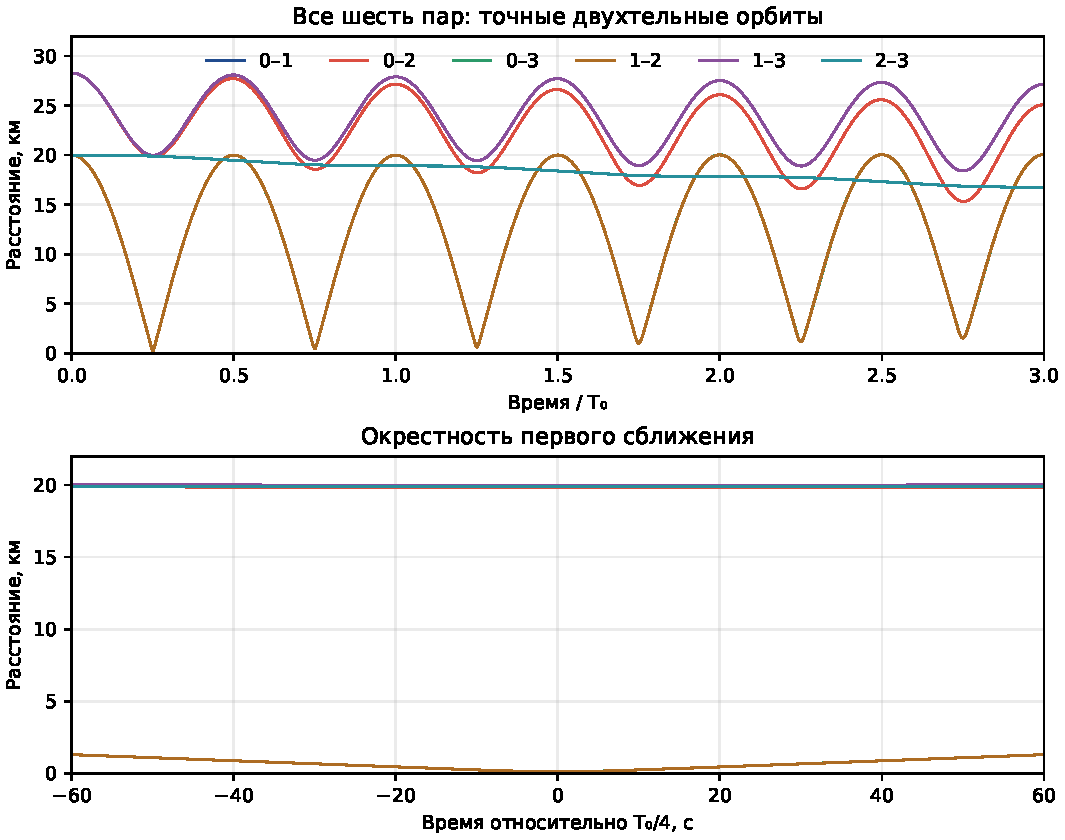
\includegraphics[width=0.94\linewidth]{two_body_distances.pdf}
\caption{Расстояния всех шести пар в независимой двухтельной
проверке пробного начального состояния. Нижняя панель
увеличивает первую окрестность $T_0/4$. Рисунок создан
скриптом \texttt{scripts/make\_two\_body\_figure.py};
он не является траекторией действующего HCW-провайдера.}
\label{fig:two_body_distances}
\end{figure}

Важно отделить четыре разных утверждения.
Повтор относительного состояния через $T_0$
выполняется для пробного набора в идеальной HCW-модели;
безопасные расстояния в ней при $T_0/4$ не сохраняются.
В точной двухтельной проверке полного повтора уже нет,
хотя расстояния двух критических пар в $T_0/4$
остаются близкими к нулю. Сохранение пространственного
квадрата на всём витке не следует ни из повторения
концов, ни из отсутствия векового члена. Наконец,
даже повтор пространственной конфигурации
не означал бы повтор угловой картинки при вращении
наземного наблюдателя.

\section{Фактический прогон демонстрации и следующий этап}
\label{sec:next_stage}

Один конкретный запуск текущего кода для исходного JSON
из табл.~\ref{tab:implementation_parameters} использует
$\theta=\arctan(20/630)=1{,}8183029644518331^\circ$,
$181$ узел от $-450$ до $450$~с с шагом $5$~с.
Таблица~\ref{tab:demo_run} получена функцией
\texttt{calculate\_free\_variants} и
\texttt{visibility\_summary}; она относится к
аналитическому HCW-провайдеру, а не к независимой
двухтельной проверке разд.~\ref{sec:two_body_check}.
Длительность означает связную цепочку приемлемых
узлов, содержащую $t=0$; максимумы ошибок и
минимумы расстояния относятся ко всему
показываемому интервалу.

\begin{table}[htbp]
\centering\scriptsize
\caption{Фактический прогон трёх вариантов одного сценария}
\label{tab:demo_run}
\setlength{\tabcolsep}{3pt}
\begin{tabular}{lcccccc}
\toprule
Вариант & Интервал, с &
Длит., с & $\max\varepsilon_b$ &
$\max\varepsilon_d$ & $\max\varepsilon_\gamma$, град &
$\min d_{ij}$, км\\
\midrule
Ориентир ОСО & $[-60,60]$ & $120$ &
$0{,}4147$ & $0{,}0925$ & $7{,}88$ & $20{,}00$\\
Пробный & $[-60,60]$ & $120$ &
$0{,}3829$ & $0{,}0995$ & $7{,}81$ & $17{,}69$\\
Подобранный & $[-215,210]$ & $425$ &
$0{,}2443$ & $0{,}0833$ & $5{,}62$ & $17{,}45$\\
\bottomrule
\end{tabular}
\end{table}

Для подобранного варианта программа выдала
$\lambda_1=629{,}838260$,
$\lambda_2=629{,}842319$,
$\lambda_3=630{,}036334$~км и модули начальных
относительных скоростей около
$42{,}14$, $46{,}84$, $4{,}75$~м/с.
На показываемом окне минимальная высота любого КА
составила $609{,}258$~км; минимум шести расстояний
$17{,}445$~км. На краях окна минимальный угол
места равен примерно $-3{,}91^\circ$, поэтому
наблюдение доступно лишь на части из $181$ отсчёта.
На этом сценарии подбор увеличил дискретно оценённую
длительность, но не является доказанной оптимизацией
и не включает стоимость формирования. Отдельная
проверка соответствующего набора начальных состояний
в абсолютной модели с $J_2$ приведена ниже;
она не превращает HCW-провайдер в нелинейный расчёт.
Ни найденное расстояние, ни положительная высота
на коротком окне не доказывают безопасность
на следующих витках.

Следующий этап --- выбирать $\lambda_i$ и начальные скорости
по допускам видимой проекции на рабочем окне и
ограничениям на все парные сближения на длинном горизонте.
Выполненный ниже один полный виток с $J_2$ является
проверкой конкретного кандидата, но не таким подбором.
При запрете тяги в рабочем окне её расход равен нулю
для всех кандидатов; выбирать следует по качеству и
длительности проекции, а также запасу расстояния.
Манёвры формирования до окна и последующие коррекции
требуют отдельной динамической модели и оценки импульса.

\section{Четыре независимые абсолютные орбиты с $J_2$}
\label{sec:j2_four_orbits}

К сценарию добавлен отдельный провайдер
\texttt{independent\_j2}. На общей эпохе
2026-09-28 00:00:00 UTC каждому из четырёх КА
заданы собственные оскулирующие элементы
$(a,e,i,\Omega,\omega,\nu)$ из
\texttt{scenarios/independent\_j2\_4sat.json}.
Их численные значения получены преобразованием
начальных инерциальных состояний подобранного
HCW-варианта; после эпохи каждый КА движется
самостоятельно и без тяги. Для круговой начальной
орбиты КА~0 направление перигея неопределённо:
в таблице принято $\omega_0=0$, а $\nu_0$
равно аргументу широты. Ось~$z$ условной ECI
совпадает с осью вращения Земли, а гринвичский
угол на эпохе принят нулевым. Указанная дата
не задаёт точной эфемеридной ориентации осей.

\begin{table}[htbp]
\centering\scriptsize
\caption{Начальные оскулирующие элементы независимых орбит.
$a$ дано в километрах, углы --- в градусах}
\label{tab:j2_elements}
\setlength{\tabcolsep}{5pt}
\begin{tabular}{rcccccc}
\toprule
КА & $a$ & $e$ & $i$ & $\Omega$ & $\omega$ & $\nu$\\
\midrule
0 & $7001{,}000000$ & $0$ & $97{,}800000$ & $55{,}226225$ & $0$ & $25{,}555817$\\
1 & $6999{,}513400$ & $0{,}005588439$ & $97{,}799175$ & $55{,}225823$ & $118{,}022187$ & $267{,}697216$\\
2 & $6997{,}834906$ & $0{,}006219013$ & $97{,}877285$ & $55{,}080453$ & $120{,}092887$ & $265{,}606700$\\
3 & $6999{,}423776$ & $0{,}000659285$ & $97{,}870593$ & $55{,}077151$ & $136{,}403299$ & $249{,}132195$\\
\bottomrule
\end{tabular}
\end{table}

В принятой модели каждая абсолютная траектория
удовлетворяет $\ddot{\mathbf r}=\mathbf g_{J_2}(\mathbf r)$, где
\begin{equation}
\mathbf g_{J_2}=-\frac{\mu\mathbf r}{r^3}
+\frac{3J_2\mu R_E^2}{2r^5}
\begin{pmatrix}
x(5z^2/r^2-1)\\ y(5z^2/r^2-1)\\ z(5z^2/r^2-3)
\end{pmatrix}.
\end{equation}
Использованы $R_E=6371$~км,
$\mu=398600{,}4$~км$^3$/с$^2$,
$J_2=0{,}00108262668$. Метод Рунге--Кутты
четвёртого порядка ограничен шагом $2$~с.
ОСО пересчитывается по фактическим
$\mathbf r_0,\mathbf v_0$; наземная проекция
и критерии квадрата вычисляются общим расчётным
слоем программы. Гравитационное ускорение
не является приложенной тягой: $\Delta v=0$
в показываемом окне.

Окно $[-450,450]$~с содержит $181$ узел.
В момент $t=0$ максимальная ошибка заданных
гномонических координат равна $6{,}4\cdot10^{-15}$.
При прежних порогах $\varepsilon_b\leq0{,}1$,
$\varepsilon_d\leq0{,}1$,
$\varepsilon_\gamma\leq10^\circ$ и
$h_i\geq15^\circ$ для всех КА допустимы
$86$ узлов; связный интервал вокруг эпохи
равен $[-215,210]$~с, то есть $425$~с.
На всём показываемом окне максимумы трёх
ошибок равны $0{,}24436$, $0{,}08285$ и
$5{,}581^\circ$; минимальный угол места
равен $-3{,}914^\circ$. Эти максимумы
включают неприемлемые края окна.

Отдельная проверка расстояний длится от $0$
до $T_0=2\pi\sqrt{a_0^3/\mu}=5829{,}765956$~с.
Это номинальный двухтельный период начального
КА~0, а не точный период модели с $J_2$.
Все шесть расстояний взяты на сетке не грубее
$5$~с. Для каждого локального минимума
найден нуль скалярного произведения
$(\mathbf r_i-\mathbf r_j)\cdot
(\mathbf v_i-\mathbf v_j)$ между узлами;
при бисекции состояние заново интегрируется
с шагом не более $0{,}1$~с.
В табл.~\ref{tab:j2_minima} широта и долгота
относятся к геоцентрической подспутниковой
точке середины пары в принятой вращающейся
системе. Максимальная широта опорного КА
по модулю на горизонте составляет $82{,}19^\circ$.

\begin{table}[htbp]
\centering\small
\caption{Уточнённые минимумы всех пар на одном номинальном витке с $J_2$}
\label{tab:j2_minima}
\begin{tabular}{ccrrr}
\toprule
Пара & $t_{\min}$, с & $d_{\min}$, км & Широта, град & Долгота, град\\
\midrule
0--1 & $2{,}290$ & $19{,}995048$ & $25{,}52$ & $51{,}47$\\
0--2 & $3{,}109$ & $28{,}276992$ & $25{,}56$ & $51{,}36$\\
0--3 & $1260{,}342$ & $9{,}704325$ & $74{,}55$ & $-100{,}21$\\
1--2 & $1280{,}324$ & $10{,}194464$ & $72{,}87$ & $-103{,}62$\\
1--3 & $5818{,}014$ & $27{,}309319$ & $24{,}77$ & $27{,}27$\\
2--3 & $2{,}053$ & $19{,}995558$ & $25{,}48$ & $51{,}29$\\
\bottomrule
\end{tabular}
\end{table}

Ни один локальный минимум не оказался ниже
настроенного иллюстративного порога $1$~км;
поэтому в этом сценарии опасных событий по
данному правилу не обнаружено. Два наиболее
тесных сближения происходят на высоких широтах.
При повторном расчёте с шагами интегрирования,
сетки и уточнения $1$, $2{,}5$ и $0{,}05$~с
соответственно расхождение конечных положений
не превысило $2{,}2\cdot10^{-8}$~км, а
расхождение парных минимумов ---
$1{,}3\cdot10^{-10}$~км. Для удельной энергии
$E=v^2/2-\mu/r+\mu J_2R_E^2(3z^2/r^2-1)/(2r^3)$
максимальный относительный дрейф составил
$1{,}15\cdot10^{-14}$.
Эти оценки относятся
к численной сходимости заданной модели и
одного витка. Они не доказывают долгосрочную
безопасность, не включают неопределённость
начальных состояний и не меняют вывод о
сближении пробного HCW-квадрата в независимой
двухтельной проверке.
\section{Обобщение одного пролёта на сетку $N\times N$}
\label{sec:grid_n}

Провайдер \texttt{independent\_j2} допускает
$2\leq N\leq10$, $S=N^2$ и опорный индекс~0.
Для строки $r$ снизу вверх и столбца $c$
слева направо постоянный индекс равен
\begin{equation}
I_N(r,c)=
\begin{cases}
rN+c, & r\ \text{чётное},\\
rN+(N-1-c), & r\ \text{нечётное}.
\end{cases}
\qquad 0\leq r,c<N.
\end{equation}
При $N=2$ индексы равны
$\bigl(\begin{smallmatrix}0&1\\3&2\end{smallmatrix}\bigr)$:
обход $0$--$1$--$2$--$3$ сохраняется.
Для любого $N$ углы перечисляются как
$I_N(0,0)$, $I_N(0,N-1)$,
$I_N(N-1,N-1)$, $I_N(N-1,0)$.

Для $u=c/(N-1)$, $v=r/(N-1)$,
$\alpha=\tan\theta$ целевые точки равны
$(\xi^*_{rc},\eta^*_{rc})=(\alpha u,\alpha v)$.
JSON задаёт четыре угловые орбиты. Только их
начальные дальности и инерциальные скорости
смешиваются с билинейными весами $w_j(u,v)$:
\begin{equation}
\lambda_{rc}=\sum_{j=0}^{3}w_j\lambda_j,
\qquad
\mathbf r_{rc}(0)=\mathbf r_{\rm obs}(0)+
\lambda_{rc}(\mathbf s_0+\alpha u\mathbf e_\xi+
\alpha v\mathbf e_\eta),
\qquad
\mathbf v_{rc}(0)=\sum_{j=0}^{3}w_j\mathbf v_j(0).
\end{equation}
Исходные угловые состояния сохраняются точно.
Из каждого нового начального состояния получают
собственные оскулирующие элементы, затем все
$S$ орбит независимо распространяют в $J_2$
без тяги. Интерполяции готовых траекторий и
оптимизации сетки нет.

\begin{table}[htbp]
\centering\small
\caption{Проверенные сетки на одном окне $[-450,450]$~с.
Расстояние относится к полному номинальному витку с $J_2$}
\label{tab:grid_results}
\begin{tabular}{rrrrccc}
\toprule
$N$ & КА & Пар & Узлов принято & Интервал, с & Длительность, с & $\min d_{ij}$, км\\
\midrule
2 & 4 & 6 & 86 & $[-215,210]$ & 425 & $9{,}704325$\\
3 & 9 & 36 & 64 & $[-95,90]$ & 185 & $4{,}834755$\\
10 & 100 & 4950 & 12 & $[-30,25]$ & 55 & $1{,}071374$\\
\bottomrule
\end{tabular}
\end{table}

Критерии исходного внешнего квадрата из
разд.~\ref{sec:implementation} применяются к
указанным четырём углам. Для $N=2$ они дают
тот же результат, что прежний четырёхточечный
провайдер. При $N>2$ дополнительно проверяются
все внутренние точки, соседние отрезки и
$(N-1)^2$ ячеек. В каждом узле действительная
проекция и угол места нужны для каждого КА.
Истинный угловой шаг соседей измеряется
не по картинной плоскости, а по единичным
направлениям визирования:
\begin{equation}
\delta_{ij}=\arccos\bigl(\operatorname{clip}
(\mathbf s_i\cdot\mathbf s_j,-1,1)\bigr),
\qquad (i,j)\in E_N,
\end{equation}
где $E_N$ состоит из всех горизонтальных и
вертикальных соседей. Принимается
$\min_{E_N}\delta_{ij}\geq\delta_{\min}$.

Отклонение внутренней точки от регулярной сетки
не зависит от общего масштаба и ориентации.
Пусть $q_{rc}=u+{\rm i}v$,
$z_{rc}=\xi_{rc}+{\rm i}\eta_{rc}$,
черта означает среднее по всем $N^2$ точкам.
Комплексный коэффициент наименьших квадратов
и нормированная максимальная ошибка равны
\begin{equation}
A=\frac{\sum_{rc}\overline{(q_{rc}-\bar q)}
(z_{rc}-\bar z)}{\sum_{rc}|q_{rc}-\bar q|^2},
\qquad
\varepsilon_{\rm point}=
\frac{\max_{rc}|z_{rc}-\bar z-A(q_{rc}-\bar q)|}
{|A|/(N-1)}.
\end{equation}
Если $\ell_e$ --- гномонические длины всех
соседних отрезков, то
$\varepsilon_{\rm step}=\max_e|\ell_e-\bar\ell|/
\bar\ell$. По формулам сторон, диагоналей и
углов разд.~\ref{sec:shape_criteria} отдельно
получают максимум трёх ошибок по всем ячейкам.
Также требуется положительное направление
каждого шага строки и столбца и выпуклость
каждой ячейки. В текущем сценарии границы для
$\varepsilon_{\rm point}$,
$\varepsilon_{\rm step}$, ошибок сторон и
диагоналей ячейки равны $0{,}1$,
для угла ячейки $10^\circ$, а
$\delta_{\min}=0{,}1^\circ$; все они находятся
в JSON и допускают изменение.

Для проверки сближений всех $S(S-1)/2$ пар
рассчитывается полный номинальный виток
$[0,T_0]$, включая широты до $82{,}19^\circ$
по модулю. При $S=4$ минимумы уточняются
описанной выше бисекцией с интегрированием $J_2$.
При большем $S$ пары обрабатываются блоками:
смена знака $\Delta\mathbf r\cdot\Delta\mathbf v$
выделяет внутренний минимум, кубический полином
Эрмита по положениям и скоростям двух узлов
уточняет его время. Если оценка оказывается
не далее $0{,}1$~км от порога $1$~км,
эта пара вновь интегрируется в $J_2$ с шагом
не более $0{,}1$~с, а время корректируется
по $\Delta\mathbf r\cdot\Delta\mathbf v=0$.
Для $N=10$ так проверены все $4950$ пар.
Для всего пролёта выбирается самый длинный связный
допустимый интервал. Сетка не грубее $5$~с может пропустить
два экстремума внутри шага без смены знака
на концах. Аудит $N>2$ идёт в фоне с явным
статусом незавершённой проверки.

Ближайшие пары для $N=3$ и $10$ ---
$5$--$6$ при $t=1261{,}694$~с на широте
$74{,}46^\circ$ и $80$--$99$ при
$t=1262{,}747$~с на широте $74{,}39^\circ$.
Последний минимум уточнён в $J_2$; его запас
над порогом $1$~км лишь $0{,}071374$~км.
Опасных событий по этому порогу не найдено.
При истинном шаге $1^\circ$ остаётся $205$~с
только у $N=2$, а при $2^\circ$ допустимых
узлов нет. Элементы и показатели сохранены в
\texttt{docs/grid\_checks/grid\_n2.json},
\texttt{grid\_n3.json}, \texttt{grid\_n10.json};
все $4950$ минимумов --- в
\texttt{grid\_n10\_pair\_minima.csv}.

\section{Отдельный обзор пассивных орбит и повторных пролётов}

В папке \texttt{orbit\_study/} выполнен ограниченный обзор
пассивных оскулирующих орбит, не меняющий работу графической
демонстрации одного пролёта. При выборе области опорных высот
учитывались методы анализа кратных трасс, условий наблюдения
и возмущённой эволюции из книги А.~А.~Чернова и
Г.~М.~Чернявского «Орбиты спутников дистанционного зондирования
Земли» (2004, гл.~4--5, 8). Периодичность подспутниковой
трассы опорного аппарата здесь используется лишь для выбора
кандидата и не принимается за доказательство периодичности
изображения всей группы.

На общей условной эпохе 28.09.2026 00:00:00 UTC
состояния каждого из $S=N^2$ КА восстановлены из собственных
\emph{оскулирующих} элементов $(a,e,i,\Omega,\omega,\nu)$
в геоцентрической инерциальной системе с осью $E_Z$ вдоль оси
вращения Земли и нулевым гринвичским углом на эпохе. Прямое
кеплерово преобразование элементов задаёт только мгновенные
$(\mathbf r_i,\mathbf v_i)$; затем каждый КА независимо
распространяется в одной нелинейной модели с $J_2$ и без тяги.
Варианты высоты $500$, $600$, $630$ и $700$~км, внешней
стороны от $2^\circ$ до $20^\circ$, фазы, наклонения и
относительных скоростей составляют конечный поисковый бюджет,
а не доказательство глобального оптимума.

Для каждого момента $t$ введём булев критерий $\mathcal A_N(t;\delta_*)$.
Он истинен только если для \emph{всех} КА определена проекция,
\begin{equation}
 h_i(t)=\arcsin\frac{(\mathbf r_i-\mathbf R)\cdot\mathbf R}
 {\|\mathbf r_i-\mathbf R\|R_E}\geq15^\circ,\qquad i=0,\ldots,S-1,
\end{equation}
внешний контур удовлетворяет прежним пределам
$\varepsilon_b,\varepsilon_d\leq0{,}1$,
$\varepsilon_\gamma\leq10^\circ$ и выпуклости, а при $N>2$
выполнены условия порядка строк и столбцов, выпуклости всех
ячеек, нормированного отклонения узлов и неравномерности
соседних шагов не более $0{,}1$, а также тех же пределов
для сторон, диагоналей и углов каждой ячейки. Отдельно
проверяется истинное, а не гномоническое расстояние между
каждой парой соседних направлений:
\begin{equation}
 \delta_{ij}(t)=\arccos(\mathbf s_i\cdot\mathbf s_j)
 \geq\delta_*,\qquad (i,j)\in E_N,\quad
 \delta_*\in\{1^\circ,2^\circ\}.
\end{equation}
Пределы формы сохранены из \eqref{eq:shape_errors} и предыдущего
обобщения решётки; порог $\delta_*$ не подменяет размер
внешнего квадрата. Последний отдельно измеряется как
$\theta_{\rm ext}(t)=\arctan\bar b(t)$, где $\bar b$
--- средняя из четырёх гномонических сторон. Для связного
принятого интервала $I=[t_a,t_b]$ сообщаются $t_a,t_b$,
$T_I=t_b-t_a$ и диапазон $[\min_I\theta_{\rm ext},
\max_I\theta_{\rm ext}]$. Численный минимум в текущем
расчёте относится к узлам не грубее $5$~с и не является
аналитической оценкой между ними.

За фактически выполненный горизонт подсчитываются отдельные
пролёты с положительным $T_I$, расстояния по времени между
их серединами и срок от первого до последнего. Для каждой
из $S(S-1)/2$ пар проверяется
\begin{equation}
 d_{ij}^{\min}=\min_{t\in H}\|\mathbf r_i(t)-\mathbf r_j(t)\|.
\end{equation}
Сетка проверки не грубее $60$~с, шаг интегрирования не более
$10$~с; внутренние экстремумы уточняются по относительным
положениям и скоростям полиномом Эрмита. Около порога и для
глобального минимума пара повторно интегрируется в $J_2$
с шагом до $0{,}1$~с. Условные геометрическая сумма радиусов
$0{,}02$~км и дополнительный запас $1{,}0$~км являются
двумя разными параметрами; неизвестные реальные габариты
и ошибки орбит не позволяют заявлять безусловную безопасность.
Численный поиск экстремумов не даёт строгого доказательства
отсутствия короткого события между узлами.
В расчёте дополнительно отмечается снижение любого КА ниже
условных $300$~км: при таком исходе тридцатисуточная
экстраполяция только с $J_2$ без атмосферы не считается
физически достоверной.

В сохранённом обзоре каждый размер $N=2,\ldots,10$ имеет
по $25$ допустимых пробных начальных наборов. Табл.~\ref{tab:passive_study}
показывает один выбранный по произведению длительности
первого пролёта и его минимальной внешней стороны кандидат.
Длительность $T_2$ относится к порогу истинного шага
$2^\circ$, а $d_{\min}$ --- ко всему указанному горизонту.
Это ограниченный обзор, не сертификат оптимальности.

\begin{table}[ht]
\centering
\small
\caption{Пассивные варианты $N\times N$ в нелинейной модели $J_2$}
\label{tab:passive_study}
\begin{tabular}{rrrrrr}
\toprule
$N$ & Горизонт, сут & Подходящих пролётов & $T_2$, с &
$\min_I\theta_{\rm ext}$, град & $d_{\min}$, км\\
\midrule
2 & 30 & 1 & 280 & $8{,}410$ & $36{,}567$\\
3 & 30 & 1 & 405 & $4{,}360$ & $1{,}287$\\
4 & 30 & 1 & 130 & $7{,}661$ & $1{,}475$\\
5 & 1  & 1 & 85  & $9{,}068$ & $0{,}218$\\
6 & 30 & 1 & 25  & $19{,}502$ & $0{,}381$\\
7 & 1  & 1 & 20  & $19{,}502$ & $0{,}290$\\
8 & 1  & 1 & 15  & $19{,}776$ & $1{,}019$\\
9 & 1  & 0 & 0   & --- & $0{,}0066$\\
10& 1  & 0 & 0   & --- & $0{,}0615$\\
\bottomrule
\end{tabular}
\end{table}

При исходно условных $0{,}02$~км для геометрической суммы
радиусов КА и дополнительном запасе $1{,}0$~км требуется
$d_{\min}\geq1{,}02$~км. На фактически просчитанном горизонте
варианты $N=5,6,7,8,9,10$ этого требования не выполняют;
для $N=9$ минимум $0{,}0066$~км нарушает и геометрический
порог. У $N=6$ за первые сутки минимум составлял
$1{,}259$~км, однако к $t=1294905{,}161$~с пара
$27$--$28$ сблизилась до $0{,}381$~км. Это демонстрирует,
почему безопасность нельзя выводить из одного витка или
одного пролёта. У $N=2,6,7,8$ минимальная высота ниже
$300$~км. На полном 30-суточном горизонте $N=2,3,4,6$
повторного принятого пролёта ни при $1^\circ$, ни при
$2^\circ$ не найдено. Для остальных размеров срок
повторяемости после первых суток не установлен. Полные
элементы на общей эпохе, события сближений и машинные
показатели находятся в \texttt{orbit\_study/results/}.
Для крупных размеров дополнительно проверены отдельные
полярные варианты $N=9,10$ с наклонением $97{,}8^\circ$ на
суточном горизонте: при достижении опорным КА широт до
$82{,}19^\circ$ по модулю минимумы всех пар составили
$0{,}070397$ и $0{,}149616$~км соответственно. Оба
нарушают принятый запас; порог различимости $2^\circ$
не даёт принятого интервала. Эти варианты сохранены
отдельно от строк табл.~\ref{tab:passive_study}.

\subsection{Использование сохранённых орбит в демонстрации}

Существующее окно использует пассивные наборы
табл.~\ref{tab:passive_study} в пункте ``Без управления''. Для заданного $N=2,\ldots,10$ из
\texttt{orbit\_study/results/solutions.json} загружаются все $N^2$
начальных оскулирующих элементов на эпохе
\texttt{2026-09-28T00:00:00Z}; мгновенные состояния преобразуются
из элементов и каждый КА вновь распространяется без тяги в модели
$J_2$. Окно показывает один пролёт $-450\ldots+450$~с относительно
этой эпохи. Для порога истинного угла соседей $1^\circ$ либо
$2^\circ$ отдельно вычисляются видимость всей сетки, принятие
формы и длительность связного интервала. На экране показываются
текущая внешняя сторона $\theta_{\rm ext}$, минимальный истинный
угол соседей, ошибки формы и расстояние между аппаратами.

Запись исследования содержит минимум всех пар за фактически
проверенный горизонт, время и геоцентрическое место события. Эти
сведения выводятся отдельно от мгновенной картины. Статус
``требования выполнены'' требует двух принятых пролётов за базовые
$30$ суток, $d_{\min}\geq1{,}02$~км и минимальной высоты
не ниже $300$~км. При отсутствии принятого пролёта для выбранного
порога или при $d_{\min}<0{,}02$~км указывается отсутствие
проверенного решения; прочие неполные случаи отмечаются как
частично выполненные. Поэтому отдельный зелёный интервал в окне
не является заключением о повторяемости и безопасности.

Совместимость сохранённого набора контролируется версией модели,
контрольной суммой используемых численных определений, содержимого
файла решений и сравнением исходных параметров с текущим сценарием.
Повторный анализ выбранного набора на новом горизонте вызывается
отдельно и сохраняет графики и численные данные в собственную папку;
в основном окне графики дальнейших пролётов отсутствуют. При
изменении физики или допусков прежние результаты не предъявляются
как результат новой модели.

\subsection{Центрированная локальная система и точный выбор размера}

На нынешнем этапе начало локальной относительной системы помещено в
геометрический центр $S=N^2$ КА, то есть в расчётную точку
\begin{equation}
 \mathbf r_c=S^{-1}\sum_{j=0}^{S-1}\mathbf r_j,\qquad
 \mathbf v_c=S^{-1}\sum_{j=0}^{S-1}\mathbf v_j.
\end{equation}
Ориентация осей по-прежнему определяется мгновенным абсолютным
состоянием назначенного опорного КА~0:
$\mathbf e_x=\mathbf r_0/|\mathbf r_0|$,
$\mathbf e_z=(\mathbf r_0\times\mathbf v_0)/|\mathbf r_0\times\mathbf v_0|$,
$\mathbf e_y=\mathbf e_z\times\mathbf e_x$. При
$B=[\mathbf e_x,\mathbf e_y,\mathbf e_z]$ относительные координаты
и скорости вычисляются как
\begin{equation}
 \boldsymbol\rho_j=B^T(\mathbf r_j-\mathbf r_c),\qquad
 \dot{\boldsymbol\rho}_j=B^T(\mathbf v_j-\mathbf v_c)
       +\dot B^T(\mathbf r_j-\mathbf r_c).
\end{equation}
Производная $\dot B$ получается из $\mathbf r_0,\mathbf v_0$ и
ускорения $J_2$. Центр не интегрируется как отдельная кеплерова
орбита. Видимая проекция вычисляется только из абсолютных
$\mathbf r_j$ и положения наблюдателя, поэтому перенос локального
начала не изменяет её; это проверено сравнением двух вариантов начала.

Заданная $\theta$ относится ко \emph{внешнему} целевому контуру:
$\alpha=\tan\theta$, а узел строки $r$ и столбца $c$ имеет
гномонические координаты $(\alpha c/(N-1),\alpha r/(N-1))$.
Фактический внешний размер определён одинаково для всех $N$ как
$\theta_{\rm ext}=\arctan[(b_0+b_1+b_2+b_3)/4]$; это не
минимальный истинный угловой шаг соседей. Пространственные размеры
в километрах также считаются отдельно: минимум и максимум соседних
сторон, четыре крайние стороны и две диагонали, минимум и максимум
среди всех пар.

При открытии окна выбраны $N=10$ и $\theta=20^\circ$; верхняя
граница поля равна $30^\circ$. Для $N=10,20^\circ$ в сохранённом
исследовании нет проверенного набора элементов: строка $N=10$
табл.~\ref{tab:passive_study} относится к $10^\circ$. При
несовпадении выбранной стороны элементы не подставляются и окно
сообщает о необходимости нового подбора. Пункт ``С управлением''
пока сообщает об отсутствии совместимого расчёта; исторический
управляемый CSV оставлен только для сравнения в репозитории.

\end{document}
